% A workaround to allow relative paths in included subfiles
% that are to be compiled separately
% See https://tex.stackexchange.com/questions/153312/subfiles-inside-a-subfile-using-relative-paths
\providecommand{\main}{..}
\documentclass[\main/thesis.tex]{subfiles}

\begin{document}

\chapter{Evaluation}
\label{cha:evaluation}
This chapter presents an evaluation of the implementation developed in \rcha{method}.
The results presented also represent one of the first evaluations of \gls{power10}'s \gls{mma} facility.
Given that the evaluation was performed on first-silicon version of \gls{power10} which runs at a lower frequency than will be featured in commercially available versions, the results are representative of the hardware that will eventually be available to consumers but performance of the commercial machines will be different.
Changes between this version and the commercial versions includes clock frequency, firmware updates or even silicon updates.

\section{Experimental Setup}
This section presents details on resources used and processes performed to produce the results in \rsec{caveats} and onwards.

\subsection{Machine Details}
The experimental platform is a \gls{power10} machine provided by \gls{ibm}.
The processor is not yet available to the public but relevant details are presented in \rtab{machineInfo}.
The listed core counts are per socket while the thread counts are per core.
The machine runs Linux with a 64-bit kernel at version 5.10.0-17496-g41bc5268c5e8.

\begin{table}[t]
  \centering
  \begin{tabular}{c | c}
    & IBM POWER10\\\hline
    Cores/Threads & 15/8\\
    L1i cache & 720KiB\\
    L1d cache & 480KiB\\
    Frequency & 3.65 GHz\\
  \end{tabular}
  \caption{POWER10 machine info.}
  \label{tab:machineInfo}
\end{table}

\subsection{Compilation}
All binaries are compiled with Clang version 13.0.0\footnotemark at the highest optimisation level (\code{-O3}) and are tuned to the processor (\code{-mcpu=pwr10}).
\footnotetext{At time of writing this is a development version.}
Because support for \gls{power10} was not available in mainstream \gls{llvm} when this work began, it has been implemented as part of \glslink{ibm}{IBM's} variant of \gls{llvm} which did have support for \gls{mma} instructions.
This variant contains several platform specific, targeted optimisations focused on improving \gls{power} code; all these specific optimizations have been disabled so that results are representative of mainstream \gls{llvm}.

\subsection{Experimental Methodology}
\begin{figure}[t]
  \centering
  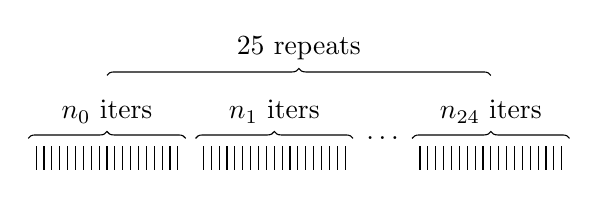
\begin{tikzpicture}[scale=1]
    \draw[decorate, decoration={brace}, align=center, shift={(0, 0)}] (0, 0) -- node[above=2] {$n_0$ iters} +(2, 0);
    \draw[decorate, decoration={brace}, align=center, shift={(2.125, 0)}] (0, 0) -- node[above=2] {$n_1$ iters} +(2, 0);
    \node[shift={(4.5, 0)}] {$\ldots$};
    \draw[decorate, decoration={brace}, align=center, shift={(4.875, 0)}] (0, 0) -- node[above=2] {$n_{24}$ iters} +(2, 0);
    \draw[decorate, decoration={brace}, align=center, shift={(1, .8)}] (0, 0) -- node[above=2] {25 repeats} +(4.875, 0);
    \foreach \x in { 0, 2.125, 4.875 }
    {
      \pgfmathsetmacro{\xStart}{\x + 0.1}
      \foreach \i in {0,...,18}
      {
        \draw[shift={(\xStart + \i * 0.1, -0.1)}] (0, 0) -- +(0, -0.3);
      }
    }
  \end{tikzpicture}
  \caption{Experiment execution process.}
  \label{fig:execution}
\end{figure}

Every measurement presented in this chapter was produced using the Google\texttrademark{} benchmark library\footnotemark~\autocite{googlebench}.
\footnotetext{At commit ab74ae5e104f72fa957c1712707a06a781a974a6.}
A single measurement is the result of timing the execution of a kernel many times until statistical stability is obtained.
The framework implements a method of measuring a kernel by placing it in a loop whose exit condition is dynamically determined by the benchmark being executed.
The loop will only exit when the kernel has been executed enough times.

To implement this method, a loop trip count, $n$, is determined by
\begin{enumerate*}[itemjoin={{; }}, itemjoin*={{; and }}, label=(\arabic*), after={\footnotemark.}]
  \item timing several executions of the benchmark
  \item multiplying the required time (set at one second\footnote{One second is double the default, suggested half-second time-limit.}) by $1.4$
  \item dividing by the average execution time of those executions
\end{enumerate*}
\footnotetext{This process can be verified in any upcoming table using $n \times \text{cpuTime} \approx 1.4e9$.}
The true process is more iterative and tries multiple values in order to produce a conservative estimate for benchmarks with variation in their execution times.
For the kernels studied in this chapter, which have very little variation, this is an accurate summary of the process.

\bk{Double check these numbers when they're finalised.}
While a single second may seem short, for the longest-running kernel presented (\atilde\SI{81}{\textit{\micro\second}}), this still results in roughly 17000 executions.
For the shortest-running kernel (\atilde\SI{14}{\textit{\nano\second}}), the kernel is executed nearly 100 million times.

In \rfig{execution}, producing one measurement (\ie completing $n$ iterations of the loop) corresponds to a single of the lower braces labeled ``$n_i$ iters''.
A total of 25 measurements are produced in this way, corresponding to the upper brace in \rfig{execution}, to reduce the impact of system fluctuations in any execution.
Repetitions vary $n$ slightly because the timing iterations may produce slightly different base times, changing the iteration count.

The framework presents statistics for each of the 10 loops including wall clock time, \gls{cpu} time, and cycles.
\bk{I think I can add instructions retired if it's a good idea.}
It also presents overall statistics between each of the ten runs: mean, median, and standard deviation.
These overall statistics are the values presented throughout the coming sections.
Vertical bars in plots represent the overall mean while error bars represent the 95\% confidence interval derived from the standard deviation.
Tables accompany each plot with execution count ($n$), mean \gls{cpu} time, mean cycles, and their respective confidence intervals.

\subsection{Types Missing From Analysis}
Three types are missing from the following analysis for different reasons.
The \code{i4} and \code{bfloat} types use the same \gls{ir} code generation code paths as every other type except \code{double}.
Given that the implemented logic works for \code{i8}, \code{i16}, \code{half}, and \code{float}, it is likely that the code generated for them is functional and as performant as the other types.
However, while translating to assembly, the backend produces either incorrect code (\code{i4}) or an error (\code{bfloat}).
Both issues have been acknowledged by the developer team and will be fixed in future versions of \gls{llvm}.

For \code{double}, the changed operation dimensions cause a signficant divergence in code generation logic that otherwise applies to all other types usable with \gls{mma}.
Due to the constraints of the surrounding framework, it was decided early on that development efforts should be focused on an algorithm that worked for six of the seven types.
The method presented in \rcha{method} can easily be applied to \code{float} but its \gls{lowering} implementation will be a noticeable variant of the original code.

\section{Caveats}
\label{sec:caveats}
The results presented in \todo{link future results section} are unexpected and less than ideal.
However, the cause of the lackluster performance, in general, is not a result of the implementation presented in \rcha{method}.
Instead, missed performance can be traced to several factors in the backend code generator as well as limitations inherent in the surrounding framework.

Before presenting the results, this section explains sources of performance degradations.
The results are counterintuitive, but the issues they reveal are addressable in the future and represent opportunities for improving code generation for the entire \gls{power} software stack.
The presented \gls{mma} kernel is a new type of kernel never before seen by the backend and therefore the assembly code generation has not been as tuned as other kernels have been.
Only after stripping away certain bottlenecks present in the naive kernel can we learn about new issues that are still to be addressed by the backend design team.

\subsection{Spilling}
In compiler terminology, a \gls{live} value is a value that may be used by a statement in the future.
Ideally, once a value is brought from memory into a register or it is computed and placed into a register, it should remain in the register until it is \gls{dead} --- a value is dead when it is guaranteed that it will never be used again.
However, there are often not enough registers available in an architecture to keep all live values in register.
Therefore, the compiler performs analysis to decide how to judiciously select some live values to be temporarily \glslink{spill}{spilled} to memory in order to temporarily free registers for new values.
Thus, \glslink{spill}{spilling} occurs when new values must be brought from memory but all registers at that \gls{point} in the program have a \gls{live} value.
For small matrix-multiplication kernels, all values may be resident in register simultaneously or may only be used once and thus do no remain \gls{live} across future loads.
Efficient spilling requires careful scheduling but in the case of \gls{mma} the problem is made more difficult by the following issues.

\subsubsection{Framework Vector Loads}
The implementation described in \rcha{method} is integrated within a pre-existing framework that provides the default vectorisation lowering method described in \rsec{matMulInt}.
This framework contains data structures to support operations with matrices.
These data structures transform the load of a single long vector representing a flattened matrix into several vector loads representing the matrix's column or row vectors, depending on the original access order.
For example, a floating-point column-major matrix \mat{A}{4}{2} is originally represented by \code{<8 x float>} and then transformed into two \code{<4 x float>} column-vector loads.
After the transformation, these load instructions in the \gls{ir} remain consecutive and occur before any computation.
An examination of the assembly code generated by the backend reveals that such a program is translated by the backend into assembly that brings \emph{all} of the matrix's elements to registers immediately and consecutively.
Given that
\begin{enumerate*}[itemjoin={{; }}, itemjoin*={{; or }}, label=(\arabic*), after={,}]
  \item the matrix may be larger than all available registers
  \item some registers may contain values from other matrices
\end{enumerate*}
many of the loaded values are immediately \glslink{spill}{spilled} back to memory.
These values must be reloaded later when they are needed, effectively tripling the time spent on memory accesses.
Memory operations are considerably slower than \gls{mma} operations, even though the values may be going to and from the L1 cache, and thus the runtime of the kernel becomes dominated by memory operations.

\begin{figure}[t]
  \centering
  %% Creator: Matplotlib, PGF backend
%%
%% To include the figure in your LaTeX document, write
%%   \input{<filename>.pgf}
%%
%% Make sure the required packages are loaded in your preamble
%%   \usepackage{pgf}
%%
%% Figures using additional raster images can only be included by \input if
%% they are in the same directory as the main LaTeX file. For loading figures
%% from other directories you can use the `import` package
%%   \usepackage{import}
%%
%% and then include the figures with
%%   \import{<path to file>}{<filename>.pgf}
%%
%% Matplotlib used the following preamble
%%
\begingroup%
\makeatletter%
\begin{pgfpicture}%
\pgfpathrectangle{\pgfpointorigin}{\pgfqpoint{5.501070in}{3.000000in}}%
\pgfusepath{use as bounding box, clip}%
\begin{pgfscope}%
\pgfsetbuttcap%
\pgfsetmiterjoin%
\definecolor{currentfill}{rgb}{1.000000,1.000000,1.000000}%
\pgfsetfillcolor{currentfill}%
\pgfsetlinewidth{0.000000pt}%
\definecolor{currentstroke}{rgb}{1.000000,1.000000,1.000000}%
\pgfsetstrokecolor{currentstroke}%
\pgfsetdash{}{0pt}%
\pgfpathmoveto{\pgfqpoint{0.000000in}{0.000000in}}%
\pgfpathlineto{\pgfqpoint{5.501070in}{0.000000in}}%
\pgfpathlineto{\pgfqpoint{5.501070in}{3.000000in}}%
\pgfpathlineto{\pgfqpoint{0.000000in}{3.000000in}}%
\pgfpathclose%
\pgfusepath{fill}%
\end{pgfscope}%
\begin{pgfscope}%
\pgfsetbuttcap%
\pgfsetmiterjoin%
\definecolor{currentfill}{rgb}{1.000000,1.000000,1.000000}%
\pgfsetfillcolor{currentfill}%
\pgfsetlinewidth{0.000000pt}%
\definecolor{currentstroke}{rgb}{0.000000,0.000000,0.000000}%
\pgfsetstrokecolor{currentstroke}%
\pgfsetstrokeopacity{0.000000}%
\pgfsetdash{}{0pt}%
\pgfpathmoveto{\pgfqpoint{0.794291in}{0.549691in}}%
\pgfpathlineto{\pgfqpoint{5.351070in}{0.549691in}}%
\pgfpathlineto{\pgfqpoint{5.351070in}{2.650926in}}%
\pgfpathlineto{\pgfqpoint{0.794291in}{2.650926in}}%
\pgfpathclose%
\pgfusepath{fill}%
\end{pgfscope}%
\begin{pgfscope}%
\pgfpathrectangle{\pgfqpoint{0.794291in}{0.549691in}}{\pgfqpoint{4.556779in}{2.101235in}}%
\pgfusepath{clip}%
\pgfsetbuttcap%
\pgfsetmiterjoin%
\definecolor{currentfill}{rgb}{0.121569,0.466667,0.705882}%
\pgfsetfillcolor{currentfill}%
\pgfsetlinewidth{0.000000pt}%
\definecolor{currentstroke}{rgb}{0.000000,0.000000,0.000000}%
\pgfsetstrokecolor{currentstroke}%
\pgfsetstrokeopacity{0.000000}%
\pgfsetdash{}{0pt}%
\pgfpathmoveto{\pgfqpoint{0.794291in}{0.549691in}}%
\pgfpathlineto{\pgfqpoint{1.687777in}{0.549691in}}%
\pgfpathlineto{\pgfqpoint{1.687777in}{0.822306in}}%
\pgfpathlineto{\pgfqpoint{0.794291in}{0.822306in}}%
\pgfpathclose%
\pgfusepath{fill}%
\end{pgfscope}%
\begin{pgfscope}%
\pgfpathrectangle{\pgfqpoint{0.794291in}{0.549691in}}{\pgfqpoint{4.556779in}{2.101235in}}%
\pgfusepath{clip}%
\pgfsetbuttcap%
\pgfsetmiterjoin%
\definecolor{currentfill}{rgb}{0.121569,0.466667,0.705882}%
\pgfsetfillcolor{currentfill}%
\pgfsetlinewidth{0.000000pt}%
\definecolor{currentstroke}{rgb}{0.000000,0.000000,0.000000}%
\pgfsetstrokecolor{currentstroke}%
\pgfsetstrokeopacity{0.000000}%
\pgfsetdash{}{0pt}%
\pgfpathmoveto{\pgfqpoint{3.296052in}{0.549691in}}%
\pgfpathlineto{\pgfqpoint{4.189538in}{0.549691in}}%
\pgfpathlineto{\pgfqpoint{4.189538in}{2.254402in}}%
\pgfpathlineto{\pgfqpoint{3.296052in}{2.254402in}}%
\pgfpathclose%
\pgfusepath{fill}%
\end{pgfscope}%
\begin{pgfscope}%
\pgfpathrectangle{\pgfqpoint{0.794291in}{0.549691in}}{\pgfqpoint{4.556779in}{2.101235in}}%
\pgfusepath{clip}%
\pgfsetbuttcap%
\pgfsetmiterjoin%
\definecolor{currentfill}{rgb}{1.000000,0.498039,0.054902}%
\pgfsetfillcolor{currentfill}%
\pgfsetlinewidth{0.000000pt}%
\definecolor{currentstroke}{rgb}{0.000000,0.000000,0.000000}%
\pgfsetstrokecolor{currentstroke}%
\pgfsetstrokeopacity{0.000000}%
\pgfsetdash{}{0pt}%
\pgfpathmoveto{\pgfqpoint{1.687777in}{0.549691in}}%
\pgfpathlineto{\pgfqpoint{2.581263in}{0.549691in}}%
\pgfpathlineto{\pgfqpoint{2.581263in}{0.618132in}}%
\pgfpathlineto{\pgfqpoint{1.687777in}{0.618132in}}%
\pgfpathclose%
\pgfusepath{fill}%
\end{pgfscope}%
\begin{pgfscope}%
\pgfpathrectangle{\pgfqpoint{0.794291in}{0.549691in}}{\pgfqpoint{4.556779in}{2.101235in}}%
\pgfusepath{clip}%
\pgfsetbuttcap%
\pgfsetmiterjoin%
\definecolor{currentfill}{rgb}{1.000000,0.498039,0.054902}%
\pgfsetfillcolor{currentfill}%
\pgfsetlinewidth{0.000000pt}%
\definecolor{currentstroke}{rgb}{0.000000,0.000000,0.000000}%
\pgfsetstrokecolor{currentstroke}%
\pgfsetstrokeopacity{0.000000}%
\pgfsetdash{}{0pt}%
\pgfpathmoveto{\pgfqpoint{4.189538in}{0.549691in}}%
\pgfpathlineto{\pgfqpoint{5.083024in}{0.549691in}}%
\pgfpathlineto{\pgfqpoint{5.083024in}{2.459905in}}%
\pgfpathlineto{\pgfqpoint{4.189538in}{2.459905in}}%
\pgfpathclose%
\pgfusepath{fill}%
\end{pgfscope}%
\begin{pgfscope}%
\pgfsetbuttcap%
\pgfsetroundjoin%
\definecolor{currentfill}{rgb}{0.000000,0.000000,0.000000}%
\pgfsetfillcolor{currentfill}%
\pgfsetlinewidth{0.803000pt}%
\definecolor{currentstroke}{rgb}{0.000000,0.000000,0.000000}%
\pgfsetstrokecolor{currentstroke}%
\pgfsetdash{}{0pt}%
\pgfsys@defobject{currentmarker}{\pgfqpoint{0.000000in}{-0.048611in}}{\pgfqpoint{0.000000in}{0.000000in}}{%
\pgfpathmoveto{\pgfqpoint{0.000000in}{0.000000in}}%
\pgfpathlineto{\pgfqpoint{0.000000in}{-0.048611in}}%
\pgfusepath{stroke,fill}%
}%
\begin{pgfscope}%
\pgfsys@transformshift{1.687777in}{0.549691in}%
\pgfsys@useobject{currentmarker}{}%
\end{pgfscope}%
\end{pgfscope}%
\begin{pgfscope}%
\definecolor{textcolor}{rgb}{0.000000,0.000000,0.000000}%
\pgfsetstrokecolor{textcolor}%
\pgfsetfillcolor{textcolor}%
\pgftext[x=1.687777in,y=0.452469in,,top]{\color{textcolor}\rmfamily\fontsize{10.000000}{12.000000}\selectfont 8x8x16}%
\end{pgfscope}%
\begin{pgfscope}%
\pgfsetbuttcap%
\pgfsetroundjoin%
\definecolor{currentfill}{rgb}{0.000000,0.000000,0.000000}%
\pgfsetfillcolor{currentfill}%
\pgfsetlinewidth{0.803000pt}%
\definecolor{currentstroke}{rgb}{0.000000,0.000000,0.000000}%
\pgfsetstrokecolor{currentstroke}%
\pgfsetdash{}{0pt}%
\pgfsys@defobject{currentmarker}{\pgfqpoint{0.000000in}{-0.048611in}}{\pgfqpoint{0.000000in}{0.000000in}}{%
\pgfpathmoveto{\pgfqpoint{0.000000in}{0.000000in}}%
\pgfpathlineto{\pgfqpoint{0.000000in}{-0.048611in}}%
\pgfusepath{stroke,fill}%
}%
\begin{pgfscope}%
\pgfsys@transformshift{4.189538in}{0.549691in}%
\pgfsys@useobject{currentmarker}{}%
\end{pgfscope}%
\end{pgfscope}%
\begin{pgfscope}%
\definecolor{textcolor}{rgb}{0.000000,0.000000,0.000000}%
\pgfsetstrokecolor{textcolor}%
\pgfsetfillcolor{textcolor}%
\pgftext[x=4.189538in,y=0.452469in,,top]{\color{textcolor}\rmfamily\fontsize{10.000000}{12.000000}\selectfont 32x8x32}%
\end{pgfscope}%
\begin{pgfscope}%
\definecolor{textcolor}{rgb}{0.000000,0.000000,0.000000}%
\pgfsetstrokecolor{textcolor}%
\pgfsetfillcolor{textcolor}%
\pgftext[x=3.072680in,y=0.273457in,,top]{\color{textcolor}\rmfamily\fontsize{10.000000}{12.000000}\selectfont Kernel Size}%
\end{pgfscope}%
\begin{pgfscope}%
\pgfsetbuttcap%
\pgfsetroundjoin%
\definecolor{currentfill}{rgb}{0.000000,0.000000,0.000000}%
\pgfsetfillcolor{currentfill}%
\pgfsetlinewidth{0.803000pt}%
\definecolor{currentstroke}{rgb}{0.000000,0.000000,0.000000}%
\pgfsetstrokecolor{currentstroke}%
\pgfsetdash{}{0pt}%
\pgfsys@defobject{currentmarker}{\pgfqpoint{-0.048611in}{0.000000in}}{\pgfqpoint{-0.000000in}{0.000000in}}{%
\pgfpathmoveto{\pgfqpoint{-0.000000in}{0.000000in}}%
\pgfpathlineto{\pgfqpoint{-0.048611in}{0.000000in}}%
\pgfusepath{stroke,fill}%
}%
\begin{pgfscope}%
\pgfsys@transformshift{0.794291in}{0.549691in}%
\pgfsys@useobject{currentmarker}{}%
\end{pgfscope}%
\end{pgfscope}%
\begin{pgfscope}%
\definecolor{textcolor}{rgb}{0.000000,0.000000,0.000000}%
\pgfsetstrokecolor{textcolor}%
\pgfsetfillcolor{textcolor}%
\pgftext[x=0.627624in, y=0.501466in, left, base]{\color{textcolor}\rmfamily\fontsize{10.000000}{12.000000}\selectfont \(\displaystyle {0}\)}%
\end{pgfscope}%
\begin{pgfscope}%
\pgfsetbuttcap%
\pgfsetroundjoin%
\definecolor{currentfill}{rgb}{0.000000,0.000000,0.000000}%
\pgfsetfillcolor{currentfill}%
\pgfsetlinewidth{0.803000pt}%
\definecolor{currentstroke}{rgb}{0.000000,0.000000,0.000000}%
\pgfsetstrokecolor{currentstroke}%
\pgfsetdash{}{0pt}%
\pgfsys@defobject{currentmarker}{\pgfqpoint{-0.048611in}{0.000000in}}{\pgfqpoint{-0.000000in}{0.000000in}}{%
\pgfpathmoveto{\pgfqpoint{-0.000000in}{0.000000in}}%
\pgfpathlineto{\pgfqpoint{-0.048611in}{0.000000in}}%
\pgfusepath{stroke,fill}%
}%
\begin{pgfscope}%
\pgfsys@transformshift{0.794291in}{1.077645in}%
\pgfsys@useobject{currentmarker}{}%
\end{pgfscope}%
\end{pgfscope}%
\begin{pgfscope}%
\definecolor{textcolor}{rgb}{0.000000,0.000000,0.000000}%
\pgfsetstrokecolor{textcolor}%
\pgfsetfillcolor{textcolor}%
\pgftext[x=0.488734in, y=1.029419in, left, base]{\color{textcolor}\rmfamily\fontsize{10.000000}{12.000000}\selectfont \(\displaystyle {220}\)}%
\end{pgfscope}%
\begin{pgfscope}%
\pgfsetbuttcap%
\pgfsetroundjoin%
\definecolor{currentfill}{rgb}{0.000000,0.000000,0.000000}%
\pgfsetfillcolor{currentfill}%
\pgfsetlinewidth{0.803000pt}%
\definecolor{currentstroke}{rgb}{0.000000,0.000000,0.000000}%
\pgfsetstrokecolor{currentstroke}%
\pgfsetdash{}{0pt}%
\pgfsys@defobject{currentmarker}{\pgfqpoint{-0.048611in}{0.000000in}}{\pgfqpoint{-0.000000in}{0.000000in}}{%
\pgfpathmoveto{\pgfqpoint{-0.000000in}{0.000000in}}%
\pgfpathlineto{\pgfqpoint{-0.048611in}{0.000000in}}%
\pgfusepath{stroke,fill}%
}%
\begin{pgfscope}%
\pgfsys@transformshift{0.794291in}{1.605598in}%
\pgfsys@useobject{currentmarker}{}%
\end{pgfscope}%
\end{pgfscope}%
\begin{pgfscope}%
\definecolor{textcolor}{rgb}{0.000000,0.000000,0.000000}%
\pgfsetstrokecolor{textcolor}%
\pgfsetfillcolor{textcolor}%
\pgftext[x=0.488734in, y=1.557373in, left, base]{\color{textcolor}\rmfamily\fontsize{10.000000}{12.000000}\selectfont \(\displaystyle {440}\)}%
\end{pgfscope}%
\begin{pgfscope}%
\pgfsetbuttcap%
\pgfsetroundjoin%
\definecolor{currentfill}{rgb}{0.000000,0.000000,0.000000}%
\pgfsetfillcolor{currentfill}%
\pgfsetlinewidth{0.803000pt}%
\definecolor{currentstroke}{rgb}{0.000000,0.000000,0.000000}%
\pgfsetstrokecolor{currentstroke}%
\pgfsetdash{}{0pt}%
\pgfsys@defobject{currentmarker}{\pgfqpoint{-0.048611in}{0.000000in}}{\pgfqpoint{-0.000000in}{0.000000in}}{%
\pgfpathmoveto{\pgfqpoint{-0.000000in}{0.000000in}}%
\pgfpathlineto{\pgfqpoint{-0.048611in}{0.000000in}}%
\pgfusepath{stroke,fill}%
}%
\begin{pgfscope}%
\pgfsys@transformshift{0.794291in}{2.133552in}%
\pgfsys@useobject{currentmarker}{}%
\end{pgfscope}%
\end{pgfscope}%
\begin{pgfscope}%
\definecolor{textcolor}{rgb}{0.000000,0.000000,0.000000}%
\pgfsetstrokecolor{textcolor}%
\pgfsetfillcolor{textcolor}%
\pgftext[x=0.488734in, y=2.085327in, left, base]{\color{textcolor}\rmfamily\fontsize{10.000000}{12.000000}\selectfont \(\displaystyle {660}\)}%
\end{pgfscope}%
\begin{pgfscope}%
\definecolor{textcolor}{rgb}{0.000000,0.000000,0.000000}%
\pgfsetstrokecolor{textcolor}%
\pgfsetfillcolor{textcolor}%
\pgftext[x=0.246451in, y=1.338927in, left, base,rotate=90.000000]{\color{textcolor}\rmfamily\fontsize{10.000000}{12.000000}\selectfont Runtime}%
\end{pgfscope}%
\begin{pgfscope}%
\definecolor{textcolor}{rgb}{0.000000,0.000000,0.000000}%
\pgfsetstrokecolor{textcolor}%
\pgfsetfillcolor{textcolor}%
\pgftext[x=0.398457in, y=1.480324in, left, base,rotate=90.000000]{\color{textcolor}\rmfamily\fontsize{10.000000}{12.000000}\selectfont (ns)}%
\end{pgfscope}%
\begin{pgfscope}%
\pgfpathrectangle{\pgfqpoint{0.794291in}{0.549691in}}{\pgfqpoint{4.556779in}{2.101235in}}%
\pgfusepath{clip}%
\pgfsetbuttcap%
\pgfsetroundjoin%
\pgfsetlinewidth{1.505625pt}%
\definecolor{currentstroke}{rgb}{0.000000,0.000000,0.000000}%
\pgfsetstrokecolor{currentstroke}%
\pgfsetdash{}{0pt}%
\pgfpathmoveto{\pgfqpoint{1.241034in}{0.821843in}}%
\pgfpathlineto{\pgfqpoint{1.241034in}{0.822769in}}%
\pgfusepath{stroke}%
\end{pgfscope}%
\begin{pgfscope}%
\pgfpathrectangle{\pgfqpoint{0.794291in}{0.549691in}}{\pgfqpoint{4.556779in}{2.101235in}}%
\pgfusepath{clip}%
\pgfsetbuttcap%
\pgfsetroundjoin%
\pgfsetlinewidth{1.505625pt}%
\definecolor{currentstroke}{rgb}{0.000000,0.000000,0.000000}%
\pgfsetstrokecolor{currentstroke}%
\pgfsetdash{}{0pt}%
\pgfpathmoveto{\pgfqpoint{3.742795in}{2.253898in}}%
\pgfpathlineto{\pgfqpoint{3.742795in}{2.254906in}}%
\pgfusepath{stroke}%
\end{pgfscope}%
\begin{pgfscope}%
\pgfpathrectangle{\pgfqpoint{0.794291in}{0.549691in}}{\pgfqpoint{4.556779in}{2.101235in}}%
\pgfusepath{clip}%
\pgfsetbuttcap%
\pgfsetroundjoin%
\pgfsetlinewidth{1.505625pt}%
\definecolor{currentstroke}{rgb}{0.000000,0.000000,0.000000}%
\pgfsetstrokecolor{currentstroke}%
\pgfsetdash{}{0pt}%
\pgfpathmoveto{\pgfqpoint{2.134520in}{0.617850in}}%
\pgfpathlineto{\pgfqpoint{2.134520in}{0.618414in}}%
\pgfusepath{stroke}%
\end{pgfscope}%
\begin{pgfscope}%
\pgfpathrectangle{\pgfqpoint{0.794291in}{0.549691in}}{\pgfqpoint{4.556779in}{2.101235in}}%
\pgfusepath{clip}%
\pgfsetbuttcap%
\pgfsetroundjoin%
\pgfsetlinewidth{1.505625pt}%
\definecolor{currentstroke}{rgb}{0.000000,0.000000,0.000000}%
\pgfsetstrokecolor{currentstroke}%
\pgfsetdash{}{0pt}%
\pgfpathmoveto{\pgfqpoint{4.636281in}{2.454448in}}%
\pgfpathlineto{\pgfqpoint{4.636281in}{2.465361in}}%
\pgfusepath{stroke}%
\end{pgfscope}%
\begin{pgfscope}%
\pgfpathrectangle{\pgfqpoint{0.794291in}{0.549691in}}{\pgfqpoint{4.556779in}{2.101235in}}%
\pgfusepath{clip}%
\pgfsetbuttcap%
\pgfsetroundjoin%
\definecolor{currentfill}{rgb}{0.000000,0.000000,0.000000}%
\pgfsetfillcolor{currentfill}%
\pgfsetlinewidth{1.003750pt}%
\definecolor{currentstroke}{rgb}{0.000000,0.000000,0.000000}%
\pgfsetstrokecolor{currentstroke}%
\pgfsetdash{}{0pt}%
\pgfsys@defobject{currentmarker}{\pgfqpoint{-0.010417in}{-0.000000in}}{\pgfqpoint{0.010417in}{0.000000in}}{%
\pgfpathmoveto{\pgfqpoint{0.010417in}{-0.000000in}}%
\pgfpathlineto{\pgfqpoint{-0.010417in}{0.000000in}}%
\pgfusepath{stroke,fill}%
}%
\begin{pgfscope}%
\pgfsys@transformshift{1.241034in}{0.821843in}%
\pgfsys@useobject{currentmarker}{}%
\end{pgfscope}%
\begin{pgfscope}%
\pgfsys@transformshift{3.742795in}{2.253898in}%
\pgfsys@useobject{currentmarker}{}%
\end{pgfscope}%
\end{pgfscope}%
\begin{pgfscope}%
\pgfpathrectangle{\pgfqpoint{0.794291in}{0.549691in}}{\pgfqpoint{4.556779in}{2.101235in}}%
\pgfusepath{clip}%
\pgfsetbuttcap%
\pgfsetroundjoin%
\definecolor{currentfill}{rgb}{0.000000,0.000000,0.000000}%
\pgfsetfillcolor{currentfill}%
\pgfsetlinewidth{1.003750pt}%
\definecolor{currentstroke}{rgb}{0.000000,0.000000,0.000000}%
\pgfsetstrokecolor{currentstroke}%
\pgfsetdash{}{0pt}%
\pgfsys@defobject{currentmarker}{\pgfqpoint{-0.010417in}{-0.000000in}}{\pgfqpoint{0.010417in}{0.000000in}}{%
\pgfpathmoveto{\pgfqpoint{0.010417in}{-0.000000in}}%
\pgfpathlineto{\pgfqpoint{-0.010417in}{0.000000in}}%
\pgfusepath{stroke,fill}%
}%
\begin{pgfscope}%
\pgfsys@transformshift{1.241034in}{0.822769in}%
\pgfsys@useobject{currentmarker}{}%
\end{pgfscope}%
\begin{pgfscope}%
\pgfsys@transformshift{3.742795in}{2.254906in}%
\pgfsys@useobject{currentmarker}{}%
\end{pgfscope}%
\end{pgfscope}%
\begin{pgfscope}%
\pgfpathrectangle{\pgfqpoint{0.794291in}{0.549691in}}{\pgfqpoint{4.556779in}{2.101235in}}%
\pgfusepath{clip}%
\pgfsetbuttcap%
\pgfsetroundjoin%
\definecolor{currentfill}{rgb}{0.000000,0.000000,0.000000}%
\pgfsetfillcolor{currentfill}%
\pgfsetlinewidth{1.003750pt}%
\definecolor{currentstroke}{rgb}{0.000000,0.000000,0.000000}%
\pgfsetstrokecolor{currentstroke}%
\pgfsetdash{}{0pt}%
\pgfsys@defobject{currentmarker}{\pgfqpoint{-0.010417in}{-0.000000in}}{\pgfqpoint{0.010417in}{0.000000in}}{%
\pgfpathmoveto{\pgfqpoint{0.010417in}{-0.000000in}}%
\pgfpathlineto{\pgfqpoint{-0.010417in}{0.000000in}}%
\pgfusepath{stroke,fill}%
}%
\begin{pgfscope}%
\pgfsys@transformshift{2.134520in}{0.617850in}%
\pgfsys@useobject{currentmarker}{}%
\end{pgfscope}%
\begin{pgfscope}%
\pgfsys@transformshift{4.636281in}{2.454448in}%
\pgfsys@useobject{currentmarker}{}%
\end{pgfscope}%
\end{pgfscope}%
\begin{pgfscope}%
\pgfpathrectangle{\pgfqpoint{0.794291in}{0.549691in}}{\pgfqpoint{4.556779in}{2.101235in}}%
\pgfusepath{clip}%
\pgfsetbuttcap%
\pgfsetroundjoin%
\definecolor{currentfill}{rgb}{0.000000,0.000000,0.000000}%
\pgfsetfillcolor{currentfill}%
\pgfsetlinewidth{1.003750pt}%
\definecolor{currentstroke}{rgb}{0.000000,0.000000,0.000000}%
\pgfsetstrokecolor{currentstroke}%
\pgfsetdash{}{0pt}%
\pgfsys@defobject{currentmarker}{\pgfqpoint{-0.010417in}{-0.000000in}}{\pgfqpoint{0.010417in}{0.000000in}}{%
\pgfpathmoveto{\pgfqpoint{0.010417in}{-0.000000in}}%
\pgfpathlineto{\pgfqpoint{-0.010417in}{0.000000in}}%
\pgfusepath{stroke,fill}%
}%
\begin{pgfscope}%
\pgfsys@transformshift{2.134520in}{0.618414in}%
\pgfsys@useobject{currentmarker}{}%
\end{pgfscope}%
\begin{pgfscope}%
\pgfsys@transformshift{4.636281in}{2.465361in}%
\pgfsys@useobject{currentmarker}{}%
\end{pgfscope}%
\end{pgfscope}%
\begin{pgfscope}%
\pgfsetrectcap%
\pgfsetmiterjoin%
\pgfsetlinewidth{0.803000pt}%
\definecolor{currentstroke}{rgb}{0.000000,0.000000,0.000000}%
\pgfsetstrokecolor{currentstroke}%
\pgfsetdash{}{0pt}%
\pgfpathmoveto{\pgfqpoint{0.794291in}{0.549691in}}%
\pgfpathlineto{\pgfqpoint{0.794291in}{2.650926in}}%
\pgfusepath{stroke}%
\end{pgfscope}%
\begin{pgfscope}%
\pgfsetrectcap%
\pgfsetmiterjoin%
\pgfsetlinewidth{0.803000pt}%
\definecolor{currentstroke}{rgb}{0.000000,0.000000,0.000000}%
\pgfsetstrokecolor{currentstroke}%
\pgfsetdash{}{0pt}%
\pgfpathmoveto{\pgfqpoint{5.351070in}{0.549691in}}%
\pgfpathlineto{\pgfqpoint{5.351070in}{2.650926in}}%
\pgfusepath{stroke}%
\end{pgfscope}%
\begin{pgfscope}%
\pgfsetrectcap%
\pgfsetmiterjoin%
\pgfsetlinewidth{0.803000pt}%
\definecolor{currentstroke}{rgb}{0.000000,0.000000,0.000000}%
\pgfsetstrokecolor{currentstroke}%
\pgfsetdash{}{0pt}%
\pgfpathmoveto{\pgfqpoint{0.794291in}{0.549691in}}%
\pgfpathlineto{\pgfqpoint{5.351070in}{0.549691in}}%
\pgfusepath{stroke}%
\end{pgfscope}%
\begin{pgfscope}%
\pgfsetrectcap%
\pgfsetmiterjoin%
\pgfsetlinewidth{0.803000pt}%
\definecolor{currentstroke}{rgb}{0.000000,0.000000,0.000000}%
\pgfsetstrokecolor{currentstroke}%
\pgfsetdash{}{0pt}%
\pgfpathmoveto{\pgfqpoint{0.794291in}{2.650926in}}%
\pgfpathlineto{\pgfqpoint{5.351070in}{2.650926in}}%
\pgfusepath{stroke}%
\end{pgfscope}%
\begin{pgfscope}%
\definecolor{textcolor}{rgb}{0.000000,0.000000,0.000000}%
\pgfsetstrokecolor{textcolor}%
\pgfsetfillcolor{textcolor}%
\pgftext[x=3.072680in,y=2.734260in,,base]{\color{textcolor}\rmfamily\fontsize{12.000000}{14.400000}\selectfont Effect of Load Sinking on Float Matrices}%
\end{pgfscope}%
\begin{pgfscope}%
\pgfsetbuttcap%
\pgfsetmiterjoin%
\definecolor{currentfill}{rgb}{1.000000,1.000000,1.000000}%
\pgfsetfillcolor{currentfill}%
\pgfsetfillopacity{0.800000}%
\pgfsetlinewidth{1.003750pt}%
\definecolor{currentstroke}{rgb}{0.800000,0.800000,0.800000}%
\pgfsetstrokecolor{currentstroke}%
\pgfsetstrokeopacity{0.800000}%
\pgfsetdash{}{0pt}%
\pgfpathmoveto{\pgfqpoint{0.891513in}{2.152470in}}%
\pgfpathlineto{\pgfqpoint{1.795063in}{2.152470in}}%
\pgfpathquadraticcurveto{\pgfqpoint{1.822841in}{2.152470in}}{\pgfqpoint{1.822841in}{2.180247in}}%
\pgfpathlineto{\pgfqpoint{1.822841in}{2.553704in}}%
\pgfpathquadraticcurveto{\pgfqpoint{1.822841in}{2.581482in}}{\pgfqpoint{1.795063in}{2.581482in}}%
\pgfpathlineto{\pgfqpoint{0.891513in}{2.581482in}}%
\pgfpathquadraticcurveto{\pgfqpoint{0.863735in}{2.581482in}}{\pgfqpoint{0.863735in}{2.553704in}}%
\pgfpathlineto{\pgfqpoint{0.863735in}{2.180247in}}%
\pgfpathquadraticcurveto{\pgfqpoint{0.863735in}{2.152470in}}{\pgfqpoint{0.891513in}{2.152470in}}%
\pgfpathclose%
\pgfusepath{stroke,fill}%
\end{pgfscope}%
\begin{pgfscope}%
\pgfsetbuttcap%
\pgfsetmiterjoin%
\definecolor{currentfill}{rgb}{0.121569,0.466667,0.705882}%
\pgfsetfillcolor{currentfill}%
\pgfsetlinewidth{0.000000pt}%
\definecolor{currentstroke}{rgb}{0.000000,0.000000,0.000000}%
\pgfsetstrokecolor{currentstroke}%
\pgfsetstrokeopacity{0.000000}%
\pgfsetdash{}{0pt}%
\pgfpathmoveto{\pgfqpoint{0.919291in}{2.428704in}}%
\pgfpathlineto{\pgfqpoint{1.197068in}{2.428704in}}%
\pgfpathlineto{\pgfqpoint{1.197068in}{2.525926in}}%
\pgfpathlineto{\pgfqpoint{0.919291in}{2.525926in}}%
\pgfpathclose%
\pgfusepath{fill}%
\end{pgfscope}%
\begin{pgfscope}%
\definecolor{textcolor}{rgb}{0.000000,0.000000,0.000000}%
\pgfsetstrokecolor{textcolor}%
\pgfsetfillcolor{textcolor}%
\pgftext[x=1.308180in,y=2.428704in,left,base]{\color{textcolor}\rmfamily\fontsize{10.000000}{12.000000}\selectfont No Opt}%
\end{pgfscope}%
\begin{pgfscope}%
\pgfsetbuttcap%
\pgfsetmiterjoin%
\definecolor{currentfill}{rgb}{1.000000,0.498039,0.054902}%
\pgfsetfillcolor{currentfill}%
\pgfsetlinewidth{0.000000pt}%
\definecolor{currentstroke}{rgb}{0.000000,0.000000,0.000000}%
\pgfsetstrokecolor{currentstroke}%
\pgfsetstrokeopacity{0.000000}%
\pgfsetdash{}{0pt}%
\pgfpathmoveto{\pgfqpoint{0.919291in}{2.235031in}}%
\pgfpathlineto{\pgfqpoint{1.197068in}{2.235031in}}%
\pgfpathlineto{\pgfqpoint{1.197068in}{2.332253in}}%
\pgfpathlineto{\pgfqpoint{0.919291in}{2.332253in}}%
\pgfpathclose%
\pgfusepath{fill}%
\end{pgfscope}%
\begin{pgfscope}%
\definecolor{textcolor}{rgb}{0.000000,0.000000,0.000000}%
\pgfsetstrokecolor{textcolor}%
\pgfsetfillcolor{textcolor}%
\pgftext[x=1.308180in,y=2.235031in,left,base]{\color{textcolor}\rmfamily\fontsize{10.000000}{12.000000}\selectfont Sink}%
\end{pgfscope}%
\end{pgfpicture}%
\makeatother%
\endgroup%

  \caption{The effect of load sinking on \code{float} and \code{i16} matrix multiplications.}
  \label{fig:floatSink}
\end{figure}

\begin{table}[t]
  \centering
  \makebox[\textwidth][c]{
    \begin{tabular}{| c | c | c | c |}
      \hline
      Name & $n$ & CPU Time (\SI{}{\textit{\nano\second}}) & Cycles\\\hline
      \code{float}, $8 \times 8 \times 16$, No Load Sinking & $25623185.92 \pm 623715.04$ & $54.84 \pm 1.39$ & $219.11 \pm 5.57$ \\\hline
      \code{float}, $8 \times 8 \times 16$, Load Sinking & $97308628.60 \pm 144463.04$ & $14.44 \pm 0.05$ & $57.67 \pm 0.19$ \\\hline
      \code{float}, $32 \times 8 \times 32$, No Load Sinking & $2146145.16 \pm 50283.11$ & $654.30 \pm 14.86$ & $2614.07 \pm 59.39$ \\\hline
      \code{float}, $32 \times 8 \times 32$, Load Sinking & $2352684.80 \pm 51746.61$ & $596.81 \pm 13.12$ & $2384.39 \pm 52.42$ \\\hline
      \code{i16}, $8 \times 8 \times 16$, No Load Sinking & $91419216.40 \pm 35690.47$ & $15.31 \pm 0.00$ & $61.18 \pm 0.02$ \\\hline
      \code{i16}, $8 \times 8 \times 16$, Load Sinking & $80431238.20 \pm 148030.83$ & $17.42 \pm 0.01$ & $69.61 \pm 0.03$ \\\hline
      \code{i16}, $32 \times 8 \times 32$, No Load Sinking & $3368892.16 \pm 18135.72$ & $415.63 \pm 2.21$ & $1660.53 \pm 8.85$ \\\hline
      \code{i16}, $32 \times 8 \times 32$, Load Sinking & $2230348.60 \pm 7729.44$ & $627.73 \pm 2.19$ & $2507.92 \pm 8.75$ \\\hline
    \end{tabular}
  }
  \caption{
    The effect of load sinking on \code{float} and \code{i16} matrix multiplications.
    See \rfig{floatSink} for graphical presentation.
    \bk{Is this better with just minimum iteration count?}
  }
  \label{tab:floatSink}
\end{table}

This spilling issue must be resolved by the backend scheduler\footnotemark: the scheduler needs to move loads closer to the \gls{point} in the program that contains the first use of the loaded value to reduce register pressure by using a technique called ``load sinking''.
\footnotetext{The backend design team is currently investigating how to implement this change to the scheduler.}
Load sinking may not reduce register pressure in many other programs, but in the case of this matrix-multiplication kernel it certainly does.
A workaround for the spilling resulting from unsunk loads, which can be used until the backend scheduler improves, consists of modifying the \gls{ir} by further breaking up the vector loads into smaller vector loads and sinking these smaller loads closer to the first use of the loaded values.

In preparation for the performance evaluation in this thesis, a short targeted \gls{ir} transformation was implemented using this tactic.
Its goal was to produce results that are more representative of the code that will be generated by a final production-ready backend.
Consider the pair of bars labeled ``8x8x16'' (\matmul{8}{8}{16}) for \code{float} (left) in \rfig{floatSink}.
This matrix size represents the best case scenario for such an optimisation:
\begin{enumerate*}[itemjoin={{; }}, itemjoin*={{; and }}, label={\protect\circled{\arabic*}}, after={.}]
  \item $A$'s eight-element column-vector load can be broken up into two four-element vector loads, each of which fills an entire \gls{vsr} (similar logic applies to $B$'s rows)
  \item only a single load is necessary to create an outer-product operand (rank-one update)
  \item each operand is used only once during the accumulation step ($2+4=6$ registers \gls{live} at once)
\end{enumerate*}
\bk{If plots are updated, update these numbers.}
Given such a perfect case, the runtime of the original version (labeled ``No Load Sinking'') is roughly quartered (\rtab{floatSink}, rows 1 and 2) in the optimised version (labeled ``Load Sinking'').
If the operation were to have more accumulations, then this gap would continue to grow as more and more spills would be required in the unoptimised version.

However, by examining the bars labeled ``8x8x16'' for \code{i16} (right) in \rfig{floatSink} we can see that for smaller types this optimisation actually causes a slight slow down (\rtab{floatSink}, rows 5 and 6).
This can be attributed to invalidating properties \circled{1} and \circled{2}: loading an \code{i16} operand no longer fills an entire register and two loads are necessary to create an operand for \code{i16} (rank-two update).
In fact, the assembly produced by the unoptimised version is much closer to the optimal handwritten version because it loads multiple vectors into a single register and uses these as source vectors for multiple shuffle instructions.
The ``optimised'' version loads only a single vector into a register, increasing register pressure, and uses each vector for only a single shuffle instruction.
It is only because the overall register pressure has been decreased by halving the element width that the performance of these two kernels show only a slight difference.

\subsubsection{Operand Spilling and Rematerialisation}
After addressing the load-sinking issue in this way, another, separate but related, issue appears.
As can be seen from the pair of bars labeled ``32x8x32'' for \code{float} in \rfig{floatSink}, the same fix that produced significant speedup for a smaller kernel has significantly reduced in effectiveness for a larger kernel.
An examination of the assembly reveals that the large number of loads that led to spills at the beginning of the kernel prior to sinking the loads are indeed no longer there.
However, while there are no spills throughout the body of the smaller kernel, the larger kernel has multiple spills or reloads per set of outer products.
The issue here is that, for the larger kernel, property \circled{3} no longer holds true.

Consider the example in \rfig{opReuse}.
The figure shows an example large kernel ($16 \times 32$) in the style of \rfig{intrinsic}; to illustrate how spills occur, the figure does not divide individual elements nor does it show $B$.
On the right, darker lines divide the output into blocks of accumulators while the lighter lines divide blocks into the eight accumulators as in \rfig{intrinsic}.
Each of the smaller boxes on the left represents an operand composed of four \code{float} elements used in an outer-product computation.

An example operand from $A$, highlighted by parallel diagonal lines, must be used in the accumulation of the first set of accumulators, highlighted by a crosshatch pattern.
In the computation of the smaller kernel in \rfig{floatSink}, this value is now \gls{dead}.
The larger kernel, however, must use the value again in computing the second set of accumulators, highlighted by a dotted pattern.

\begin{figure}[t]
  \centering
  \begin{tikzpicture}[scale=1/2]
    \draw[xstep=1, ystep=2, shift={(0, 0)}] (0, 0) grid +(2, 8);
    \draw[pattern=north west lines, shift={(0, 6)}] (0, 0) rectangle +(1, 2);
    \draw[pattern=crosshatch, shift={(3, 6)}] (0, 0) rectangle +(8, 2);
 %   \draw[pattern={Hatch[angle=45,distance={8pt},xshift=.2pt, line width=1.25]}, shift={(3, 6)}] (0, 0) rectangle +(8, 2);
    \draw[pattern=dots, shift={(11, 6)}] (0, 0) rectangle +(8, 2);
 %   \draw[pattern={Dots[angle=45,distance={7pt},xshift=.1pt, radius=1.25]}, shift={(11, 6)}] (0, 0) rectangle +(8, 2);
    \draw[xstep=2, ystep=2, shift={(3, 0)}, color={black!20!white}] (0, 0) grid +(16, 8);
    \draw[xstep=8, ystep=4, shift={(3, 0)}] (0, 0) grid +(16, 8);
    \draw[decorate, decoration={brace, mirror}] (0, -0.3) -- node[below=2] {$K$} +(2, 0);
  \end{tikzpicture}
  \caption{Demonstration of operand reuse.}
  \label{fig:opReuse}
\end{figure}

According to constraint \fbox{5} in \rsec{baseCase}, spilling an accumulator is expensive, and therefore an efficient solution must finish computing a block of accumulators before moving on to a different area of the matrix.
\nelson{Not clear what "before an operand" means here.}
\bk{
  Is this clear now?
  There was a typo before but I've also cleared up some other things.
}
Doing so requires that every operand along the dimension $K$ be brought to register before an operand can be reused with a new block of accumulators.
For instance, an accumulator layout like that in \rfig{opReuse} requires six operand registers for each accumulation to be performed.
Using only the 32 registers available while the accumulators are assembled, if $K \geq \left\lceil \frac{32}{6} \right\rceil = 6$, then there is not enough space for all values to remain in registers.
And thus the cause for the multiple spills and reloads throughout the computation becomes apparent: operands from $A$\footnotemark that are still \gls{live} are being forced out of registers and the compiler is choosing to spill them.
\footnotetext{The issue is identical for operands of $B$, though the reuse distance is greater.}

\bk{I've changed the discussion of rematerialisation, let me know if it's better.}
This code generation evokes the well-studied compiler technique ``\gls{rematerialisation}''.
Essentially, the compiler analysis must answer the question ``is it more efficient to store a value to memory and retrieve it later (\gls{spill}) or to recompute it later using the same process?''

In the case of floats, producing the operand is a simple load and therefore, if an operand \emph{must} be evicted from its register, \glslink{rematerialisation}{rematerialising} the value is a simple load.
Thus, the compiler's choice to spill the operand is incorrect and, because spills are saved on the stack, not only is it wasting memory by duplicating the value, it is potentially evicting values from the cache.
Regardless, the larger kernel's execution, optimised or not, is signficantly influenced by memory operations, though the gains from reducing the initial spills still have significant impact.

For smaller datatypes however, spilling is the correct choice.
Materialising an \code{i16} involves two loads and at least one instruction to shuffle the loaded data together.
Rematerialising the value in the future becomes a simple load, significantly reducing register pressure and required memory bandwidth.
Both the unoptimised and load-sinking version correctly choose to spill their values instead of \glslink{rematerialisation}{rematerialising} them.
As with \code{float}, the increased number of memory operations explains the significant increase in execution time for the larger \code{i16} kernel in \rfig{floatSink}, but it does not, however, explain the large difference between the two version.
The next section investigates this discrepancy.

\subsubsection{Smaller Types}
While the issues affecting \code{float} matrices presented above remain roughly identical for \code{double}-typed operations, small datatypes have a separate source of slow down.
The difference in performance is actually an exacerbation of an already-discussed issue, namely the invalidation of properties \circled{1} and \circled{2}.
For \code{i16}, in the load-sinking version, loads are performed four \code{i16} elements at the same time using the 64-bit doubleword load.
The unoptimised version loads 16 elements at a time using 256-bit vector-pair loads, meaning that the load-sinking version quadruples the number of ``necessary'' loads (excluding loads from the original spilling issue).
If the scheduling were fixed, removing the unnecessary loads and stores, it is likely the performance gap would be much more significant.

This issue extends to the other data types which perform rank-two, -four, or -eight updates.
The issue is aggravated as the number of memory requests increase due to shrinking data width and a greater required number of vectors for shuffling.
For example, where, for \code{i16}, the load-sinking version has roughly 114\% of the execution time of the unoptimised version, the same comparison for \code{i8} shows the load-sinking version has 292\% of the unoptimised version's execution time.

A more complicated load breaking and sinking strategy may counteract this slowdown, but only to a certain degree.
Combining certain loads -- for example two four-element \code{i16} column loads, making a full \gls{vsr} -- would decrease register pressure because the upper and lower halves of the register can be used in separate shuffles.
However, this still does not quite match the 256-bit paired-vector load in terms of memory-request efficiency.
It is impossible for smaller types to use this 256-bit load because the columns of $A$ are consecutive: the paired-vector load would load values that are not used until the second row of accumulator blocks, inevitably introducing new spills.

The issue worsens for \code{i8} and \code{i4} where the eight consecutive vertical elements fill less and less of a \gls{vsr}.
For larger kernels, the smaller data types thus imply a increasing number of loads, further diluting the speedup gained from \gls{mma}.

\subsection{Shuffling}
For datatypes smaller than 32 bits, producing the appropriate operand for a rank-$r$ update requires several vectors be merged via shuffling.
The \gls{power} \gls{isa} offers several methods to move vector elements, ranging from register shifting and rotating combined with masking to efficient vector upper and lower half merges based on datatype size.
Transforming \gls{ir} statements in an efficient code for shuffling is an involved design process.

There are a multitude ways to express the same shuffling operation in \gls{ir}, each depending on multiple implementation choices made throughout the process.
Certain variants are interpreted by the backend and translated to efficient code while others are interpreted very conservatively.
\nelson{"This"}
This can be the difference between an idiomatic assembly of several instructions, often close to an expert's handwritten version, and the same process being expressed in hundreds or thousands of instructions, often with \glspl{spill} throughout.
Several factors that lead shuffling to cause performance degradation are discussed below.

\subsubsection{Datatype: \texorpdfstring{\code{half}}{half}}
\bk{
  I think this issue is likely to affect \code{bfloat} as well but when I went to try it last night (I'd never compiled any \code{bfloat} code before) it crashed.
  I've spoken to Nemanja and it seems to be a backend issue; I've created a github issue for it and the backend team will look at it shortly.
}
\nelson{It this paragraph simply stating the currently the shuffling is incorrect?}
\bk{No, the shuffling is correct, just needlessly conservative, choosing a very roundabout method to perform the shuffles, thus making it slow.}
The \code{i16} and \code{half} types have identical widths: a halfword.
Because \glspl{cpu} and their accompanying \glspl{isa} are type-agnostic and sensitive only to the width of a data element when implementing vector shuffles, shuffle code in the \gls{ir} that differs only in choice of 16-bit type should produce identical assembly.
This is demonstrably untrue, however.
The assembly code generated for \code{i16} executes roughly six vector loads and six vector permute instructions to produce all operands for a single accumulation in a full $2 \times 4$ accumulator layout.
For \code{half}, the assembly has extended from six instructions to almost 150 and has been at least partially scalarised, moving elements from vector registers to general purpose registers and back again.

This explosion in code size is most apparent in the calculation epilogue where, in the \gls{ir}, the accumulators are disassembled and stored to memory.
First, the resulting accumulator vectors are truncated to the output data type.
They are then concatenated together into a output flattened matrix and stored to memory.
Concatenation is also achieved through shuffling and therefore experiences the same conservative code generation as before.
The added truncation operation worsens the effect.
All told, the epilogue for \code{half} is roughly ten times the length of the same operation for \code{i16}.

\subsubsection{Datatype: \texorpdfstring{\code{i4}}{i4}}
For \code{i8}, degradations arise from \glspl{spill} due to extra register pressure but also from needing to merge four separate vectors (rank-four update).
Despite this, generated code is relatively close to the ideal, handwritten assembly.
As mentioned before, there exists instructions for merging vectors at a per-byte granularity, but not a at a sub-byte granularity as is required for \code{i4} code generation in the same style.
This does not mean that it is not possible to shuffle a vector of \code{i4} elements using the same \gls{ir} code generation, only that assembly generated by the backed will be significantly less performant.
Specifically, this includes vector rotations and scalarisation, with single bytes being moved individually to and from general purpose registers.
This slow down negates much of the speed up that could be achieved via the \gls{mma} rank-eight update.

\subsection{Solutions}
This section presents potential solutions though it is unlikely that the ideas introduced will solve the performance degradations without further investigation and cooperation with the backend developers.

\subsubsection{Spilling}
\label{sec:spillSolution}
The simplest solution to the noted \glslink{spill}{spilling} issues is for developers to focus on using only small kernels and, indeed, this is not so unreasonable a proposal as one might perceive it at first.
While \gls{llvm} necessitates that certain sequences of \gls{ir} always be able to be lowered to assembly, it does not require that the code be as performant as possible, as is demonstrated by the above issues with shuffling \code{i4} vectors.
This may seem like a defeatist notion but is actually a tried-and-true approach to performance in compilers: make the common case fast.

The average user interacts with a compiler through a high-level language, not its \gls{ir}.
Thus, the frontend will choose the fastest solution to implement a user's code; if the fastest implementation is a small kernel encapsulated by an outer kernel then that is what will be chosen.
With this notion, optimisation can be focused on this most common case for which a solution is known.
A larger inner-kernel will always remain usable but it will be less performant.

Furthermore, the most performant library implementations focus on using small unrolled assembly kernels, often computing kernels with dimensions of four to eight elements.
These small kernels are then surrounded by memory-managing outer kernels as described in \rsec{outerKernel}.
This is exactly what Kuzma \etal~\autocite{kuzma2021fast} do while using the inner kernel presented in this thesis with results comparable to libraries with kernels written in assembly.
In this way, using only smaller kernels can be seen as a well-worn path to performance.

If a larger kernel \emph{must} be used, significant investigation must be done to test load scheduling, value \gls{rematerialisation}, load breaking, and, if necessary, load recombination.
It is unlikely that such a solution will be found within the \gls{ir} because .
\begin{enumerate*}[itemjoin={{; }}, itemjoin*={{; and }}, label=(\arabic*), after={.}]
  \item it is in \gls{ssa} form which often folds identical values together without consideration for the times when a value is \gls{live}
  \item for better or worse, the backend does not have to respect \gls{ir} operation order
\end{enumerate*}
Such a solution will have to be found in the backend.

\subsubsection{Shuffling}
Unlike issues with spilling, it is likely that performance degradations caused by misbehaving shuffles can be solved by creating type specific shuffling code.
While injecting the proposed solution code into the original vectorisation framework is possible, it would be much more effective to first refactor the framework so such a modification is easier.

For \code{half} vectors, it may be possible to fool the compiler into generating code as is done for \code{i16} simply by reinterpreting data as \code{i16} via casts and manipulating the data in this state.
The cast is not a conversion, simply a reinterpretation of the bits in a register, meaningful only within the \gls{llvm} framework and producing no new instructions.
The data can again be casted back to \code{half} at no cost when it needs to be used in a computation.
In theory, this produces much better assembly but may also trigger a very conservative response in the compiler, worsening the code significantly with scalar element movement derived from a perceived conversion hazard.

The sub-byte granularity of \code{i4} vectors pose a different problem.
Performant shuffling code for \code{i4} in the same style as the larger types is an impossibility.
Instead, clever use of bitwise operations will have to explicitly be used to implement efficient element extraction and movement.
Bitwise operations can be applied across an entire vector register, removing the need for scalarisation and improving register usage by reducing the number of required intermediate registers.

\subsubsection{Evaluation Disclaimer}
All evaluation presented in future sections have no targeted optimisations applied.
No tested solution positively affected all cases.
Thus, all test cases use identical \gls{ir} generation logic with no special cases.
The presented results are therefore equally advantaged and disadvantaged in code generation.

\section{Varied Access Orders}
As discussed in \rsec{outerKernel}, packing is incredibly important for matrix multiplication performance.
An important part of packing, beyond choosing dimensions, is the choice of data access order.
\rsec{registerArguments} shows that \gls{mma} is sensitive to the access order of elements in \glspl{vsr}.
This inevitably translates to a sensitivity to the access order of the matrices in memory that provide the arguments in register.

\subsection{Expectation}
\label{sec:orderExpectation}
For $A$, it is expected that data laid out in a column-major orientation is optimal.
For \code{float}, while technically a row-major matrix when in \gls{vsr}, is indistinguishable from a single column of four elements.
Thus, if $A$ is laid out in column-major order, an operand can be created with a single load and no waste.
However, if $A$ is laid out in row-major order, it is likely the case that $K \ne 1$ and thus the elements in the first column of $A$ are not consecutive in memory.
Therefore, to create an operand, four loads must be issued, one for each element of the operand.
Further overhead is incurred to move elements into the vector register either from scalar registers if the four scalar loads were issued or to shuffle elements from four vectors that were loaded.
Thus, a column-major order layout is highly preferred.
The same logic can be applied to $B$, except that a row-major orientation is preferred.

For smaller types, the logic is more complicated because the byte-length of the overall loaded data also shrinks.
In the interest of not repeating much of the discussion in \rsec{caveats}, the same logic as above can be applied while acknowledging that as register usage efficiency decreases speedups also decrease.

An interesting point of discussion exists for types \code{i8} and \code{i4} whose in-register dimensions are $4 \times 4$ and $4 \times 8$ respectively.
Because two \code{i4} elements are packed into a byte, an eight-element vector is only four bytes.
This means that both \code{i8} and \code{i4} require loading four four-byte vectors to provide the elements to fill a \gls{vsr}.
Therefore, there will always be four loads issued whether the matrix that is being extracted from has a row-major or column-major order.
In this case, it would seem that either orientation is therefore acceptable.
This is true in the case that operands are being built in isolation.
However, if one considers that several operands are being built simultaneously, loads can be combined to increase efficiency.
Shuffle instructions do not decrease, only the indices from which shuffles extract elements in a vector change.
This optimisation can have a small but noticeable impact on the results.

Naively, $C$ optimally has a row-major orientation.
This is simply because the simplest method of using \gls{mma} places the operand from $A$ as the first argument and the operand from $B$ as the second argument in the outer product instruction.
When used in this way, the elements in the accumulator are oriented in a row-major fashion and, after disassembling, there is no extra work required before storing the underlying vectors to memory.
Transposing the values so that they can be stored into a column-major output-matrix requires extra shuffles.
However, with the theorem discussed in \rsec{arbitraryOrder}, it is shown that reversing the order of the arguments causes the result in the accumulator to be equivalent but in a column-major order.
Thus, it is expected that either access order can be used for $C$ without loss of performance.

\subsection{Setup}
When using an unmodified version of \gls{llvm}, the access orders of $A$, $B$, and $C$ are tied together and must be equal.
Thus two test cases, one all-column-major ($\textrm{C} = \textrm{C} \times \textrm{C}$) and another all-row-major ($\textrm{R} = \textrm{R} \times \textrm{R}$), constitute the baseline for the experiment.
In order to test the performance of the hypothesised best mix of orientations, further modifications to the lowering framework were performed to enable the mixing of orientations.
With this possibility enabled, two cases are added to the comparison: both use the proposed optimal layout for $A$ and $B$ but vary the layout of $C$ ($\textrm{C} = \textrm{C} \times \textrm{R}$ and $\textrm{R} = \textrm{C} \times \textrm{R}$)

Each kernel uses a $2 \times 4$ accumulator setup and therefore, in keeping with the suggestion in \rsec{spillSolution}, uses a small $8 \times 16$ output.
A total of 32 accumulations are performed each kernel, making the overall computation \matmul{8}{32}{16}.
It may seem that 32 accumulations is relatively large, but~\autocite{kuzma2021fast} determines that, even given the poor load scheduling, up to 128 accumulations per kernel gives good speed up, with performance plateauing with any more accumulations.
Given the discussion in \rsec{orderExpectation}, more accumulations implies more opportunities for a ``good'' orientation to outperform a bad orientation, effectively highlighting differences in performance.

\subsection{Analysis}
\begin{figure}[t]
  \centering
  %% Creator: Matplotlib, PGF backend
%%
%% To include the figure in your LaTeX document, write
%%   \input{<filename>.pgf}
%%
%% Make sure the required packages are loaded in your preamble
%%   \usepackage{pgf}
%%
%% Figures using additional raster images can only be included by \input if
%% they are in the same directory as the main LaTeX file. For loading figures
%% from other directories you can use the `import` package
%%   \usepackage{import}
%%
%% and then include the figures with
%%   \import{<path to file>}{<filename>.pgf}
%%
%% Matplotlib used the following preamble
%%
\begingroup%
\makeatletter%
\begin{pgfpicture}%
\pgfpathrectangle{\pgfpointorigin}{\pgfqpoint{5.501070in}{5.500000in}}%
\pgfusepath{use as bounding box, clip}%
\begin{pgfscope}%
\pgfsetbuttcap%
\pgfsetmiterjoin%
\definecolor{currentfill}{rgb}{1.000000,1.000000,1.000000}%
\pgfsetfillcolor{currentfill}%
\pgfsetlinewidth{0.000000pt}%
\definecolor{currentstroke}{rgb}{1.000000,1.000000,1.000000}%
\pgfsetstrokecolor{currentstroke}%
\pgfsetdash{}{0pt}%
\pgfpathmoveto{\pgfqpoint{0.000000in}{0.000000in}}%
\pgfpathlineto{\pgfqpoint{5.501070in}{0.000000in}}%
\pgfpathlineto{\pgfqpoint{5.501070in}{5.500000in}}%
\pgfpathlineto{\pgfqpoint{0.000000in}{5.500000in}}%
\pgfpathclose%
\pgfusepath{fill}%
\end{pgfscope}%
\begin{pgfscope}%
\pgfsetbuttcap%
\pgfsetmiterjoin%
\definecolor{currentfill}{rgb}{1.000000,1.000000,1.000000}%
\pgfsetfillcolor{currentfill}%
\pgfsetlinewidth{0.000000pt}%
\definecolor{currentstroke}{rgb}{0.000000,0.000000,0.000000}%
\pgfsetstrokecolor{currentstroke}%
\pgfsetstrokeopacity{0.000000}%
\pgfsetdash{}{0pt}%
\pgfpathmoveto{\pgfqpoint{0.704013in}{3.242658in}}%
\pgfpathlineto{\pgfqpoint{2.710257in}{3.242658in}}%
\pgfpathlineto{\pgfqpoint{2.710257in}{4.852779in}}%
\pgfpathlineto{\pgfqpoint{0.704013in}{4.852779in}}%
\pgfpathclose%
\pgfusepath{fill}%
\end{pgfscope}%
\begin{pgfscope}%
\pgfpathrectangle{\pgfqpoint{0.704013in}{3.242658in}}{\pgfqpoint{2.006244in}{1.610121in}}%
\pgfusepath{clip}%
\pgfsetbuttcap%
\pgfsetmiterjoin%
\definecolor{currentfill}{rgb}{0.121569,0.466667,0.705882}%
\pgfsetfillcolor{currentfill}%
\pgfsetlinewidth{0.000000pt}%
\definecolor{currentstroke}{rgb}{0.000000,0.000000,0.000000}%
\pgfsetstrokecolor{currentstroke}%
\pgfsetstrokeopacity{0.000000}%
\pgfsetdash{}{0pt}%
\pgfpathmoveto{\pgfqpoint{0.704013in}{3.242658in}}%
\pgfpathlineto{\pgfqpoint{1.097394in}{3.242658in}}%
\pgfpathlineto{\pgfqpoint{1.097394in}{4.706404in}}%
\pgfpathlineto{\pgfqpoint{0.704013in}{4.706404in}}%
\pgfpathclose%
\pgfusepath{fill}%
\end{pgfscope}%
\begin{pgfscope}%
\pgfpathrectangle{\pgfqpoint{0.704013in}{3.242658in}}{\pgfqpoint{2.006244in}{1.610121in}}%
\pgfusepath{clip}%
\pgfsetbuttcap%
\pgfsetmiterjoin%
\definecolor{currentfill}{rgb}{0.121569,0.466667,0.705882}%
\pgfsetfillcolor{currentfill}%
\pgfsetlinewidth{0.000000pt}%
\definecolor{currentstroke}{rgb}{0.000000,0.000000,0.000000}%
\pgfsetstrokecolor{currentstroke}%
\pgfsetstrokeopacity{0.000000}%
\pgfsetdash{}{0pt}%
\pgfpathmoveto{\pgfqpoint{1.254747in}{3.242658in}}%
\pgfpathlineto{\pgfqpoint{1.648128in}{3.242658in}}%
\pgfpathlineto{\pgfqpoint{1.648128in}{4.362724in}}%
\pgfpathlineto{\pgfqpoint{1.254747in}{4.362724in}}%
\pgfpathclose%
\pgfusepath{fill}%
\end{pgfscope}%
\begin{pgfscope}%
\pgfpathrectangle{\pgfqpoint{0.704013in}{3.242658in}}{\pgfqpoint{2.006244in}{1.610121in}}%
\pgfusepath{clip}%
\pgfsetbuttcap%
\pgfsetmiterjoin%
\definecolor{currentfill}{rgb}{0.121569,0.466667,0.705882}%
\pgfsetfillcolor{currentfill}%
\pgfsetlinewidth{0.000000pt}%
\definecolor{currentstroke}{rgb}{0.000000,0.000000,0.000000}%
\pgfsetstrokecolor{currentstroke}%
\pgfsetstrokeopacity{0.000000}%
\pgfsetdash{}{0pt}%
\pgfpathmoveto{\pgfqpoint{1.805480in}{3.242658in}}%
\pgfpathlineto{\pgfqpoint{2.198862in}{3.242658in}}%
\pgfpathlineto{\pgfqpoint{2.198862in}{4.132819in}}%
\pgfpathlineto{\pgfqpoint{1.805480in}{4.132819in}}%
\pgfpathclose%
\pgfusepath{fill}%
\end{pgfscope}%
\begin{pgfscope}%
\pgfpathrectangle{\pgfqpoint{0.704013in}{3.242658in}}{\pgfqpoint{2.006244in}{1.610121in}}%
\pgfusepath{clip}%
\pgfsetbuttcap%
\pgfsetmiterjoin%
\definecolor{currentfill}{rgb}{0.121569,0.466667,0.705882}%
\pgfsetfillcolor{currentfill}%
\pgfsetlinewidth{0.000000pt}%
\definecolor{currentstroke}{rgb}{0.000000,0.000000,0.000000}%
\pgfsetstrokecolor{currentstroke}%
\pgfsetstrokeopacity{0.000000}%
\pgfsetdash{}{0pt}%
\pgfpathmoveto{\pgfqpoint{2.356214in}{3.242658in}}%
\pgfpathlineto{\pgfqpoint{2.749595in}{3.242658in}}%
\pgfpathlineto{\pgfqpoint{2.749595in}{4.113584in}}%
\pgfpathlineto{\pgfqpoint{2.356214in}{4.113584in}}%
\pgfpathclose%
\pgfusepath{fill}%
\end{pgfscope}%
\begin{pgfscope}%
\pgfsetbuttcap%
\pgfsetroundjoin%
\definecolor{currentfill}{rgb}{0.000000,0.000000,0.000000}%
\pgfsetfillcolor{currentfill}%
\pgfsetlinewidth{0.803000pt}%
\definecolor{currentstroke}{rgb}{0.000000,0.000000,0.000000}%
\pgfsetstrokecolor{currentstroke}%
\pgfsetdash{}{0pt}%
\pgfsys@defobject{currentmarker}{\pgfqpoint{0.000000in}{-0.048611in}}{\pgfqpoint{0.000000in}{0.000000in}}{%
\pgfpathmoveto{\pgfqpoint{0.000000in}{0.000000in}}%
\pgfpathlineto{\pgfqpoint{0.000000in}{-0.048611in}}%
\pgfusepath{stroke,fill}%
}%
\begin{pgfscope}%
\pgfsys@transformshift{0.900704in}{3.242658in}%
\pgfsys@useobject{currentmarker}{}%
\end{pgfscope}%
\end{pgfscope}%
\begin{pgfscope}%
\definecolor{textcolor}{rgb}{0.000000,0.000000,0.000000}%
\pgfsetstrokecolor{textcolor}%
\pgfsetfillcolor{textcolor}%
\pgftext[x=0.310200in, y=2.882522in, left, base,rotate=15.000000]{\color{textcolor}\rmfamily\fontsize{10.000000}{12.000000}\selectfont \(\displaystyle \textrm{C} = \textrm{C} \times \textrm{C}\)}%
\end{pgfscope}%
\begin{pgfscope}%
\pgfsetbuttcap%
\pgfsetroundjoin%
\definecolor{currentfill}{rgb}{0.000000,0.000000,0.000000}%
\pgfsetfillcolor{currentfill}%
\pgfsetlinewidth{0.803000pt}%
\definecolor{currentstroke}{rgb}{0.000000,0.000000,0.000000}%
\pgfsetstrokecolor{currentstroke}%
\pgfsetdash{}{0pt}%
\pgfsys@defobject{currentmarker}{\pgfqpoint{0.000000in}{-0.048611in}}{\pgfqpoint{0.000000in}{0.000000in}}{%
\pgfpathmoveto{\pgfqpoint{0.000000in}{0.000000in}}%
\pgfpathlineto{\pgfqpoint{0.000000in}{-0.048611in}}%
\pgfusepath{stroke,fill}%
}%
\begin{pgfscope}%
\pgfsys@transformshift{1.451437in}{3.242658in}%
\pgfsys@useobject{currentmarker}{}%
\end{pgfscope}%
\end{pgfscope}%
\begin{pgfscope}%
\definecolor{textcolor}{rgb}{0.000000,0.000000,0.000000}%
\pgfsetstrokecolor{textcolor}%
\pgfsetfillcolor{textcolor}%
\pgftext[x=0.855344in, y=2.881024in, left, base,rotate=15.000000]{\color{textcolor}\rmfamily\fontsize{10.000000}{12.000000}\selectfont \(\displaystyle \textrm{R} = \textrm{R} \times \textrm{R}\)}%
\end{pgfscope}%
\begin{pgfscope}%
\pgfsetbuttcap%
\pgfsetroundjoin%
\definecolor{currentfill}{rgb}{0.000000,0.000000,0.000000}%
\pgfsetfillcolor{currentfill}%
\pgfsetlinewidth{0.803000pt}%
\definecolor{currentstroke}{rgb}{0.000000,0.000000,0.000000}%
\pgfsetstrokecolor{currentstroke}%
\pgfsetdash{}{0pt}%
\pgfsys@defobject{currentmarker}{\pgfqpoint{0.000000in}{-0.048611in}}{\pgfqpoint{0.000000in}{0.000000in}}{%
\pgfpathmoveto{\pgfqpoint{0.000000in}{0.000000in}}%
\pgfpathlineto{\pgfqpoint{0.000000in}{-0.048611in}}%
\pgfusepath{stroke,fill}%
}%
\begin{pgfscope}%
\pgfsys@transformshift{2.002171in}{3.242658in}%
\pgfsys@useobject{currentmarker}{}%
\end{pgfscope}%
\end{pgfscope}%
\begin{pgfscope}%
\definecolor{textcolor}{rgb}{0.000000,0.000000,0.000000}%
\pgfsetstrokecolor{textcolor}%
\pgfsetfillcolor{textcolor}%
\pgftext[x=1.409804in, y=2.882023in, left, base,rotate=15.000000]{\color{textcolor}\rmfamily\fontsize{10.000000}{12.000000}\selectfont \(\displaystyle \textrm{C} = \textrm{C} \times \textrm{R}\)}%
\end{pgfscope}%
\begin{pgfscope}%
\pgfsetbuttcap%
\pgfsetroundjoin%
\definecolor{currentfill}{rgb}{0.000000,0.000000,0.000000}%
\pgfsetfillcolor{currentfill}%
\pgfsetlinewidth{0.803000pt}%
\definecolor{currentstroke}{rgb}{0.000000,0.000000,0.000000}%
\pgfsetstrokecolor{currentstroke}%
\pgfsetdash{}{0pt}%
\pgfsys@defobject{currentmarker}{\pgfqpoint{0.000000in}{-0.048611in}}{\pgfqpoint{0.000000in}{0.000000in}}{%
\pgfpathmoveto{\pgfqpoint{0.000000in}{0.000000in}}%
\pgfpathlineto{\pgfqpoint{0.000000in}{-0.048611in}}%
\pgfusepath{stroke,fill}%
}%
\begin{pgfscope}%
\pgfsys@transformshift{2.552905in}{3.242658in}%
\pgfsys@useobject{currentmarker}{}%
\end{pgfscope}%
\end{pgfscope}%
\begin{pgfscope}%
\definecolor{textcolor}{rgb}{0.000000,0.000000,0.000000}%
\pgfsetstrokecolor{textcolor}%
\pgfsetfillcolor{textcolor}%
\pgftext[x=1.958675in, y=2.881524in, left, base,rotate=15.000000]{\color{textcolor}\rmfamily\fontsize{10.000000}{12.000000}\selectfont \(\displaystyle \textrm{R} = \textrm{C} \times \textrm{R}\)}%
\end{pgfscope}%
\begin{pgfscope}%
\definecolor{textcolor}{rgb}{0.000000,0.000000,0.000000}%
\pgfsetstrokecolor{textcolor}%
\pgfsetfillcolor{textcolor}%
\pgftext[x=1.707135in,y=2.799383in,,top]{\color{textcolor}\rmfamily\fontsize{10.000000}{12.000000}\selectfont Matrix Access Order}%
\end{pgfscope}%
\begin{pgfscope}%
\pgfsetbuttcap%
\pgfsetroundjoin%
\definecolor{currentfill}{rgb}{0.000000,0.000000,0.000000}%
\pgfsetfillcolor{currentfill}%
\pgfsetlinewidth{0.803000pt}%
\definecolor{currentstroke}{rgb}{0.000000,0.000000,0.000000}%
\pgfsetstrokecolor{currentstroke}%
\pgfsetdash{}{0pt}%
\pgfsys@defobject{currentmarker}{\pgfqpoint{-0.048611in}{0.000000in}}{\pgfqpoint{-0.000000in}{0.000000in}}{%
\pgfpathmoveto{\pgfqpoint{-0.000000in}{0.000000in}}%
\pgfpathlineto{\pgfqpoint{-0.048611in}{0.000000in}}%
\pgfusepath{stroke,fill}%
}%
\begin{pgfscope}%
\pgfsys@transformshift{0.704013in}{3.242658in}%
\pgfsys@useobject{currentmarker}{}%
\end{pgfscope}%
\end{pgfscope}%
\begin{pgfscope}%
\definecolor{textcolor}{rgb}{0.000000,0.000000,0.000000}%
\pgfsetstrokecolor{textcolor}%
\pgfsetfillcolor{textcolor}%
\pgftext[x=0.537346in, y=3.194433in, left, base]{\color{textcolor}\rmfamily\fontsize{10.000000}{12.000000}\selectfont \(\displaystyle {0}\)}%
\end{pgfscope}%
\begin{pgfscope}%
\pgfsetbuttcap%
\pgfsetroundjoin%
\definecolor{currentfill}{rgb}{0.000000,0.000000,0.000000}%
\pgfsetfillcolor{currentfill}%
\pgfsetlinewidth{0.803000pt}%
\definecolor{currentstroke}{rgb}{0.000000,0.000000,0.000000}%
\pgfsetstrokecolor{currentstroke}%
\pgfsetdash{}{0pt}%
\pgfsys@defobject{currentmarker}{\pgfqpoint{-0.048611in}{0.000000in}}{\pgfqpoint{-0.000000in}{0.000000in}}{%
\pgfpathmoveto{\pgfqpoint{-0.000000in}{0.000000in}}%
\pgfpathlineto{\pgfqpoint{-0.048611in}{0.000000in}}%
\pgfusepath{stroke,fill}%
}%
\begin{pgfscope}%
\pgfsys@transformshift{0.704013in}{3.634326in}%
\pgfsys@useobject{currentmarker}{}%
\end{pgfscope}%
\end{pgfscope}%
\begin{pgfscope}%
\definecolor{textcolor}{rgb}{0.000000,0.000000,0.000000}%
\pgfsetstrokecolor{textcolor}%
\pgfsetfillcolor{textcolor}%
\pgftext[x=0.398457in, y=3.586101in, left, base]{\color{textcolor}\rmfamily\fontsize{10.000000}{12.000000}\selectfont \(\displaystyle {140}\)}%
\end{pgfscope}%
\begin{pgfscope}%
\pgfsetbuttcap%
\pgfsetroundjoin%
\definecolor{currentfill}{rgb}{0.000000,0.000000,0.000000}%
\pgfsetfillcolor{currentfill}%
\pgfsetlinewidth{0.803000pt}%
\definecolor{currentstroke}{rgb}{0.000000,0.000000,0.000000}%
\pgfsetstrokecolor{currentstroke}%
\pgfsetdash{}{0pt}%
\pgfsys@defobject{currentmarker}{\pgfqpoint{-0.048611in}{0.000000in}}{\pgfqpoint{-0.000000in}{0.000000in}}{%
\pgfpathmoveto{\pgfqpoint{-0.000000in}{0.000000in}}%
\pgfpathlineto{\pgfqpoint{-0.048611in}{0.000000in}}%
\pgfusepath{stroke,fill}%
}%
\begin{pgfscope}%
\pgfsys@transformshift{0.704013in}{4.025994in}%
\pgfsys@useobject{currentmarker}{}%
\end{pgfscope}%
\end{pgfscope}%
\begin{pgfscope}%
\definecolor{textcolor}{rgb}{0.000000,0.000000,0.000000}%
\pgfsetstrokecolor{textcolor}%
\pgfsetfillcolor{textcolor}%
\pgftext[x=0.398457in, y=3.977769in, left, base]{\color{textcolor}\rmfamily\fontsize{10.000000}{12.000000}\selectfont \(\displaystyle {280}\)}%
\end{pgfscope}%
\begin{pgfscope}%
\pgfsetbuttcap%
\pgfsetroundjoin%
\definecolor{currentfill}{rgb}{0.000000,0.000000,0.000000}%
\pgfsetfillcolor{currentfill}%
\pgfsetlinewidth{0.803000pt}%
\definecolor{currentstroke}{rgb}{0.000000,0.000000,0.000000}%
\pgfsetstrokecolor{currentstroke}%
\pgfsetdash{}{0pt}%
\pgfsys@defobject{currentmarker}{\pgfqpoint{-0.048611in}{0.000000in}}{\pgfqpoint{-0.000000in}{0.000000in}}{%
\pgfpathmoveto{\pgfqpoint{-0.000000in}{0.000000in}}%
\pgfpathlineto{\pgfqpoint{-0.048611in}{0.000000in}}%
\pgfusepath{stroke,fill}%
}%
\begin{pgfscope}%
\pgfsys@transformshift{0.704013in}{4.417662in}%
\pgfsys@useobject{currentmarker}{}%
\end{pgfscope}%
\end{pgfscope}%
\begin{pgfscope}%
\definecolor{textcolor}{rgb}{0.000000,0.000000,0.000000}%
\pgfsetstrokecolor{textcolor}%
\pgfsetfillcolor{textcolor}%
\pgftext[x=0.398457in, y=4.369437in, left, base]{\color{textcolor}\rmfamily\fontsize{10.000000}{12.000000}\selectfont \(\displaystyle {420}\)}%
\end{pgfscope}%
\begin{pgfscope}%
\pgfsetbuttcap%
\pgfsetroundjoin%
\definecolor{currentfill}{rgb}{0.000000,0.000000,0.000000}%
\pgfsetfillcolor{currentfill}%
\pgfsetlinewidth{0.803000pt}%
\definecolor{currentstroke}{rgb}{0.000000,0.000000,0.000000}%
\pgfsetstrokecolor{currentstroke}%
\pgfsetdash{}{0pt}%
\pgfsys@defobject{currentmarker}{\pgfqpoint{-0.048611in}{0.000000in}}{\pgfqpoint{-0.000000in}{0.000000in}}{%
\pgfpathmoveto{\pgfqpoint{-0.000000in}{0.000000in}}%
\pgfpathlineto{\pgfqpoint{-0.048611in}{0.000000in}}%
\pgfusepath{stroke,fill}%
}%
\begin{pgfscope}%
\pgfsys@transformshift{0.704013in}{4.809330in}%
\pgfsys@useobject{currentmarker}{}%
\end{pgfscope}%
\end{pgfscope}%
\begin{pgfscope}%
\definecolor{textcolor}{rgb}{0.000000,0.000000,0.000000}%
\pgfsetstrokecolor{textcolor}%
\pgfsetfillcolor{textcolor}%
\pgftext[x=0.398457in, y=4.761105in, left, base]{\color{textcolor}\rmfamily\fontsize{10.000000}{12.000000}\selectfont \(\displaystyle {560}\)}%
\end{pgfscope}%
\begin{pgfscope}%
\definecolor{textcolor}{rgb}{0.000000,0.000000,0.000000}%
\pgfsetstrokecolor{textcolor}%
\pgfsetfillcolor{textcolor}%
\pgftext[x=0.342901in,y=4.047718in,,bottom,rotate=90.000000]{\color{textcolor}\rmfamily\fontsize{10.000000}{12.000000}\selectfont Cycles}%
\end{pgfscope}%
\begin{pgfscope}%
\pgfpathrectangle{\pgfqpoint{0.704013in}{3.242658in}}{\pgfqpoint{2.006244in}{1.610121in}}%
\pgfusepath{clip}%
\pgfsetbuttcap%
\pgfsetroundjoin%
\pgfsetlinewidth{1.505625pt}%
\definecolor{currentstroke}{rgb}{0.000000,0.000000,0.000000}%
\pgfsetstrokecolor{currentstroke}%
\pgfsetdash{}{0pt}%
\pgfpathmoveto{\pgfqpoint{0.900704in}{4.701201in}}%
\pgfpathlineto{\pgfqpoint{0.900704in}{4.711607in}}%
\pgfusepath{stroke}%
\end{pgfscope}%
\begin{pgfscope}%
\pgfpathrectangle{\pgfqpoint{0.704013in}{3.242658in}}{\pgfqpoint{2.006244in}{1.610121in}}%
\pgfusepath{clip}%
\pgfsetbuttcap%
\pgfsetroundjoin%
\pgfsetlinewidth{1.505625pt}%
\definecolor{currentstroke}{rgb}{0.000000,0.000000,0.000000}%
\pgfsetstrokecolor{currentstroke}%
\pgfsetdash{}{0pt}%
\pgfpathmoveto{\pgfqpoint{1.451437in}{4.359022in}}%
\pgfpathlineto{\pgfqpoint{1.451437in}{4.366426in}}%
\pgfusepath{stroke}%
\end{pgfscope}%
\begin{pgfscope}%
\pgfpathrectangle{\pgfqpoint{0.704013in}{3.242658in}}{\pgfqpoint{2.006244in}{1.610121in}}%
\pgfusepath{clip}%
\pgfsetbuttcap%
\pgfsetroundjoin%
\pgfsetlinewidth{1.505625pt}%
\definecolor{currentstroke}{rgb}{0.000000,0.000000,0.000000}%
\pgfsetstrokecolor{currentstroke}%
\pgfsetdash{}{0pt}%
\pgfpathmoveto{\pgfqpoint{2.002171in}{4.116014in}}%
\pgfpathlineto{\pgfqpoint{2.002171in}{4.149623in}}%
\pgfusepath{stroke}%
\end{pgfscope}%
\begin{pgfscope}%
\pgfpathrectangle{\pgfqpoint{0.704013in}{3.242658in}}{\pgfqpoint{2.006244in}{1.610121in}}%
\pgfusepath{clip}%
\pgfsetbuttcap%
\pgfsetroundjoin%
\pgfsetlinewidth{1.505625pt}%
\definecolor{currentstroke}{rgb}{0.000000,0.000000,0.000000}%
\pgfsetstrokecolor{currentstroke}%
\pgfsetdash{}{0pt}%
\pgfpathmoveto{\pgfqpoint{2.552905in}{4.098994in}}%
\pgfpathlineto{\pgfqpoint{2.552905in}{4.128173in}}%
\pgfusepath{stroke}%
\end{pgfscope}%
\begin{pgfscope}%
\pgfpathrectangle{\pgfqpoint{0.704013in}{3.242658in}}{\pgfqpoint{2.006244in}{1.610121in}}%
\pgfusepath{clip}%
\pgfsetbuttcap%
\pgfsetroundjoin%
\definecolor{currentfill}{rgb}{0.000000,0.000000,0.000000}%
\pgfsetfillcolor{currentfill}%
\pgfsetlinewidth{1.003750pt}%
\definecolor{currentstroke}{rgb}{0.000000,0.000000,0.000000}%
\pgfsetstrokecolor{currentstroke}%
\pgfsetdash{}{0pt}%
\pgfsys@defobject{currentmarker}{\pgfqpoint{-0.010417in}{-0.000000in}}{\pgfqpoint{0.010417in}{0.000000in}}{%
\pgfpathmoveto{\pgfqpoint{0.010417in}{-0.000000in}}%
\pgfpathlineto{\pgfqpoint{-0.010417in}{0.000000in}}%
\pgfusepath{stroke,fill}%
}%
\begin{pgfscope}%
\pgfsys@transformshift{0.900704in}{4.701201in}%
\pgfsys@useobject{currentmarker}{}%
\end{pgfscope}%
\begin{pgfscope}%
\pgfsys@transformshift{1.451437in}{4.359022in}%
\pgfsys@useobject{currentmarker}{}%
\end{pgfscope}%
\begin{pgfscope}%
\pgfsys@transformshift{2.002171in}{4.116014in}%
\pgfsys@useobject{currentmarker}{}%
\end{pgfscope}%
\begin{pgfscope}%
\pgfsys@transformshift{2.552905in}{4.098994in}%
\pgfsys@useobject{currentmarker}{}%
\end{pgfscope}%
\end{pgfscope}%
\begin{pgfscope}%
\pgfpathrectangle{\pgfqpoint{0.704013in}{3.242658in}}{\pgfqpoint{2.006244in}{1.610121in}}%
\pgfusepath{clip}%
\pgfsetbuttcap%
\pgfsetroundjoin%
\definecolor{currentfill}{rgb}{0.000000,0.000000,0.000000}%
\pgfsetfillcolor{currentfill}%
\pgfsetlinewidth{1.003750pt}%
\definecolor{currentstroke}{rgb}{0.000000,0.000000,0.000000}%
\pgfsetstrokecolor{currentstroke}%
\pgfsetdash{}{0pt}%
\pgfsys@defobject{currentmarker}{\pgfqpoint{-0.010417in}{-0.000000in}}{\pgfqpoint{0.010417in}{0.000000in}}{%
\pgfpathmoveto{\pgfqpoint{0.010417in}{-0.000000in}}%
\pgfpathlineto{\pgfqpoint{-0.010417in}{0.000000in}}%
\pgfusepath{stroke,fill}%
}%
\begin{pgfscope}%
\pgfsys@transformshift{0.900704in}{4.711607in}%
\pgfsys@useobject{currentmarker}{}%
\end{pgfscope}%
\begin{pgfscope}%
\pgfsys@transformshift{1.451437in}{4.366426in}%
\pgfsys@useobject{currentmarker}{}%
\end{pgfscope}%
\begin{pgfscope}%
\pgfsys@transformshift{2.002171in}{4.149623in}%
\pgfsys@useobject{currentmarker}{}%
\end{pgfscope}%
\begin{pgfscope}%
\pgfsys@transformshift{2.552905in}{4.128173in}%
\pgfsys@useobject{currentmarker}{}%
\end{pgfscope}%
\end{pgfscope}%
\begin{pgfscope}%
\pgfsetrectcap%
\pgfsetmiterjoin%
\pgfsetlinewidth{0.803000pt}%
\definecolor{currentstroke}{rgb}{0.000000,0.000000,0.000000}%
\pgfsetstrokecolor{currentstroke}%
\pgfsetdash{}{0pt}%
\pgfpathmoveto{\pgfqpoint{0.704013in}{3.242658in}}%
\pgfpathlineto{\pgfqpoint{0.704013in}{4.852779in}}%
\pgfusepath{stroke}%
\end{pgfscope}%
\begin{pgfscope}%
\pgfsetrectcap%
\pgfsetmiterjoin%
\pgfsetlinewidth{0.803000pt}%
\definecolor{currentstroke}{rgb}{0.000000,0.000000,0.000000}%
\pgfsetstrokecolor{currentstroke}%
\pgfsetdash{}{0pt}%
\pgfpathmoveto{\pgfqpoint{2.710257in}{3.242658in}}%
\pgfpathlineto{\pgfqpoint{2.710257in}{4.852779in}}%
\pgfusepath{stroke}%
\end{pgfscope}%
\begin{pgfscope}%
\pgfsetrectcap%
\pgfsetmiterjoin%
\pgfsetlinewidth{0.803000pt}%
\definecolor{currentstroke}{rgb}{0.000000,0.000000,0.000000}%
\pgfsetstrokecolor{currentstroke}%
\pgfsetdash{}{0pt}%
\pgfpathmoveto{\pgfqpoint{0.704013in}{3.242658in}}%
\pgfpathlineto{\pgfqpoint{2.710257in}{3.242658in}}%
\pgfusepath{stroke}%
\end{pgfscope}%
\begin{pgfscope}%
\pgfsetrectcap%
\pgfsetmiterjoin%
\pgfsetlinewidth{0.803000pt}%
\definecolor{currentstroke}{rgb}{0.000000,0.000000,0.000000}%
\pgfsetstrokecolor{currentstroke}%
\pgfsetdash{}{0pt}%
\pgfpathmoveto{\pgfqpoint{0.704013in}{4.852779in}}%
\pgfpathlineto{\pgfqpoint{2.710257in}{4.852779in}}%
\pgfusepath{stroke}%
\end{pgfscope}%
\begin{pgfscope}%
\definecolor{textcolor}{rgb}{0.000000,0.000000,0.000000}%
\pgfsetstrokecolor{textcolor}%
\pgfsetfillcolor{textcolor}%
\pgftext[x=1.707135in,y=4.936112in,,base]{\color{textcolor}\rmfamily\fontsize{12.000000}{14.400000}\selectfont \texttt{float}}%
\end{pgfscope}%
\begin{pgfscope}%
\pgfsetbuttcap%
\pgfsetmiterjoin%
\definecolor{currentfill}{rgb}{1.000000,1.000000,1.000000}%
\pgfsetfillcolor{currentfill}%
\pgfsetlinewidth{0.000000pt}%
\definecolor{currentstroke}{rgb}{0.000000,0.000000,0.000000}%
\pgfsetstrokecolor{currentstroke}%
\pgfsetstrokeopacity{0.000000}%
\pgfsetdash{}{0pt}%
\pgfpathmoveto{\pgfqpoint{3.344826in}{3.242658in}}%
\pgfpathlineto{\pgfqpoint{5.351070in}{3.242658in}}%
\pgfpathlineto{\pgfqpoint{5.351070in}{4.852779in}}%
\pgfpathlineto{\pgfqpoint{3.344826in}{4.852779in}}%
\pgfpathclose%
\pgfusepath{fill}%
\end{pgfscope}%
\begin{pgfscope}%
\pgfpathrectangle{\pgfqpoint{3.344826in}{3.242658in}}{\pgfqpoint{2.006244in}{1.610121in}}%
\pgfusepath{clip}%
\pgfsetbuttcap%
\pgfsetmiterjoin%
\definecolor{currentfill}{rgb}{0.121569,0.466667,0.705882}%
\pgfsetfillcolor{currentfill}%
\pgfsetlinewidth{0.000000pt}%
\definecolor{currentstroke}{rgb}{0.000000,0.000000,0.000000}%
\pgfsetstrokecolor{currentstroke}%
\pgfsetstrokeopacity{0.000000}%
\pgfsetdash{}{0pt}%
\pgfpathmoveto{\pgfqpoint{3.344826in}{3.242658in}}%
\pgfpathlineto{\pgfqpoint{3.738207in}{3.242658in}}%
\pgfpathlineto{\pgfqpoint{3.738207in}{4.706404in}}%
\pgfpathlineto{\pgfqpoint{3.344826in}{4.706404in}}%
\pgfpathclose%
\pgfusepath{fill}%
\end{pgfscope}%
\begin{pgfscope}%
\pgfpathrectangle{\pgfqpoint{3.344826in}{3.242658in}}{\pgfqpoint{2.006244in}{1.610121in}}%
\pgfusepath{clip}%
\pgfsetbuttcap%
\pgfsetmiterjoin%
\definecolor{currentfill}{rgb}{0.121569,0.466667,0.705882}%
\pgfsetfillcolor{currentfill}%
\pgfsetlinewidth{0.000000pt}%
\definecolor{currentstroke}{rgb}{0.000000,0.000000,0.000000}%
\pgfsetstrokecolor{currentstroke}%
\pgfsetstrokeopacity{0.000000}%
\pgfsetdash{}{0pt}%
\pgfpathmoveto{\pgfqpoint{3.895559in}{3.242658in}}%
\pgfpathlineto{\pgfqpoint{4.288941in}{3.242658in}}%
\pgfpathlineto{\pgfqpoint{4.288941in}{4.404653in}}%
\pgfpathlineto{\pgfqpoint{3.895559in}{4.404653in}}%
\pgfpathclose%
\pgfusepath{fill}%
\end{pgfscope}%
\begin{pgfscope}%
\pgfpathrectangle{\pgfqpoint{3.344826in}{3.242658in}}{\pgfqpoint{2.006244in}{1.610121in}}%
\pgfusepath{clip}%
\pgfsetbuttcap%
\pgfsetmiterjoin%
\definecolor{currentfill}{rgb}{0.121569,0.466667,0.705882}%
\pgfsetfillcolor{currentfill}%
\pgfsetlinewidth{0.000000pt}%
\definecolor{currentstroke}{rgb}{0.000000,0.000000,0.000000}%
\pgfsetstrokecolor{currentstroke}%
\pgfsetstrokeopacity{0.000000}%
\pgfsetdash{}{0pt}%
\pgfpathmoveto{\pgfqpoint{4.446293in}{3.242658in}}%
\pgfpathlineto{\pgfqpoint{4.839674in}{3.242658in}}%
\pgfpathlineto{\pgfqpoint{4.839674in}{4.263239in}}%
\pgfpathlineto{\pgfqpoint{4.446293in}{4.263239in}}%
\pgfpathclose%
\pgfusepath{fill}%
\end{pgfscope}%
\begin{pgfscope}%
\pgfpathrectangle{\pgfqpoint{3.344826in}{3.242658in}}{\pgfqpoint{2.006244in}{1.610121in}}%
\pgfusepath{clip}%
\pgfsetbuttcap%
\pgfsetmiterjoin%
\definecolor{currentfill}{rgb}{0.121569,0.466667,0.705882}%
\pgfsetfillcolor{currentfill}%
\pgfsetlinewidth{0.000000pt}%
\definecolor{currentstroke}{rgb}{0.000000,0.000000,0.000000}%
\pgfsetstrokecolor{currentstroke}%
\pgfsetstrokeopacity{0.000000}%
\pgfsetdash{}{0pt}%
\pgfpathmoveto{\pgfqpoint{4.997027in}{3.242658in}}%
\pgfpathlineto{\pgfqpoint{5.390408in}{3.242658in}}%
\pgfpathlineto{\pgfqpoint{5.390408in}{4.262469in}}%
\pgfpathlineto{\pgfqpoint{4.997027in}{4.262469in}}%
\pgfpathclose%
\pgfusepath{fill}%
\end{pgfscope}%
\begin{pgfscope}%
\pgfsetbuttcap%
\pgfsetroundjoin%
\definecolor{currentfill}{rgb}{0.000000,0.000000,0.000000}%
\pgfsetfillcolor{currentfill}%
\pgfsetlinewidth{0.803000pt}%
\definecolor{currentstroke}{rgb}{0.000000,0.000000,0.000000}%
\pgfsetstrokecolor{currentstroke}%
\pgfsetdash{}{0pt}%
\pgfsys@defobject{currentmarker}{\pgfqpoint{0.000000in}{-0.048611in}}{\pgfqpoint{0.000000in}{0.000000in}}{%
\pgfpathmoveto{\pgfqpoint{0.000000in}{0.000000in}}%
\pgfpathlineto{\pgfqpoint{0.000000in}{-0.048611in}}%
\pgfusepath{stroke,fill}%
}%
\begin{pgfscope}%
\pgfsys@transformshift{3.541516in}{3.242658in}%
\pgfsys@useobject{currentmarker}{}%
\end{pgfscope}%
\end{pgfscope}%
\begin{pgfscope}%
\definecolor{textcolor}{rgb}{0.000000,0.000000,0.000000}%
\pgfsetstrokecolor{textcolor}%
\pgfsetfillcolor{textcolor}%
\pgftext[x=2.951013in, y=2.882522in, left, base,rotate=15.000000]{\color{textcolor}\rmfamily\fontsize{10.000000}{12.000000}\selectfont \(\displaystyle \textrm{C} = \textrm{C} \times \textrm{C}\)}%
\end{pgfscope}%
\begin{pgfscope}%
\pgfsetbuttcap%
\pgfsetroundjoin%
\definecolor{currentfill}{rgb}{0.000000,0.000000,0.000000}%
\pgfsetfillcolor{currentfill}%
\pgfsetlinewidth{0.803000pt}%
\definecolor{currentstroke}{rgb}{0.000000,0.000000,0.000000}%
\pgfsetstrokecolor{currentstroke}%
\pgfsetdash{}{0pt}%
\pgfsys@defobject{currentmarker}{\pgfqpoint{0.000000in}{-0.048611in}}{\pgfqpoint{0.000000in}{0.000000in}}{%
\pgfpathmoveto{\pgfqpoint{0.000000in}{0.000000in}}%
\pgfpathlineto{\pgfqpoint{0.000000in}{-0.048611in}}%
\pgfusepath{stroke,fill}%
}%
\begin{pgfscope}%
\pgfsys@transformshift{4.092250in}{3.242658in}%
\pgfsys@useobject{currentmarker}{}%
\end{pgfscope}%
\end{pgfscope}%
\begin{pgfscope}%
\definecolor{textcolor}{rgb}{0.000000,0.000000,0.000000}%
\pgfsetstrokecolor{textcolor}%
\pgfsetfillcolor{textcolor}%
\pgftext[x=3.496157in, y=2.881024in, left, base,rotate=15.000000]{\color{textcolor}\rmfamily\fontsize{10.000000}{12.000000}\selectfont \(\displaystyle \textrm{R} = \textrm{R} \times \textrm{R}\)}%
\end{pgfscope}%
\begin{pgfscope}%
\pgfsetbuttcap%
\pgfsetroundjoin%
\definecolor{currentfill}{rgb}{0.000000,0.000000,0.000000}%
\pgfsetfillcolor{currentfill}%
\pgfsetlinewidth{0.803000pt}%
\definecolor{currentstroke}{rgb}{0.000000,0.000000,0.000000}%
\pgfsetstrokecolor{currentstroke}%
\pgfsetdash{}{0pt}%
\pgfsys@defobject{currentmarker}{\pgfqpoint{0.000000in}{-0.048611in}}{\pgfqpoint{0.000000in}{0.000000in}}{%
\pgfpathmoveto{\pgfqpoint{0.000000in}{0.000000in}}%
\pgfpathlineto{\pgfqpoint{0.000000in}{-0.048611in}}%
\pgfusepath{stroke,fill}%
}%
\begin{pgfscope}%
\pgfsys@transformshift{4.642984in}{3.242658in}%
\pgfsys@useobject{currentmarker}{}%
\end{pgfscope}%
\end{pgfscope}%
\begin{pgfscope}%
\definecolor{textcolor}{rgb}{0.000000,0.000000,0.000000}%
\pgfsetstrokecolor{textcolor}%
\pgfsetfillcolor{textcolor}%
\pgftext[x=4.050617in, y=2.882023in, left, base,rotate=15.000000]{\color{textcolor}\rmfamily\fontsize{10.000000}{12.000000}\selectfont \(\displaystyle \textrm{C} = \textrm{C} \times \textrm{R}\)}%
\end{pgfscope}%
\begin{pgfscope}%
\pgfsetbuttcap%
\pgfsetroundjoin%
\definecolor{currentfill}{rgb}{0.000000,0.000000,0.000000}%
\pgfsetfillcolor{currentfill}%
\pgfsetlinewidth{0.803000pt}%
\definecolor{currentstroke}{rgb}{0.000000,0.000000,0.000000}%
\pgfsetstrokecolor{currentstroke}%
\pgfsetdash{}{0pt}%
\pgfsys@defobject{currentmarker}{\pgfqpoint{0.000000in}{-0.048611in}}{\pgfqpoint{0.000000in}{0.000000in}}{%
\pgfpathmoveto{\pgfqpoint{0.000000in}{0.000000in}}%
\pgfpathlineto{\pgfqpoint{0.000000in}{-0.048611in}}%
\pgfusepath{stroke,fill}%
}%
\begin{pgfscope}%
\pgfsys@transformshift{5.193718in}{3.242658in}%
\pgfsys@useobject{currentmarker}{}%
\end{pgfscope}%
\end{pgfscope}%
\begin{pgfscope}%
\definecolor{textcolor}{rgb}{0.000000,0.000000,0.000000}%
\pgfsetstrokecolor{textcolor}%
\pgfsetfillcolor{textcolor}%
\pgftext[x=4.599487in, y=2.881524in, left, base,rotate=15.000000]{\color{textcolor}\rmfamily\fontsize{10.000000}{12.000000}\selectfont \(\displaystyle \textrm{R} = \textrm{C} \times \textrm{R}\)}%
\end{pgfscope}%
\begin{pgfscope}%
\definecolor{textcolor}{rgb}{0.000000,0.000000,0.000000}%
\pgfsetstrokecolor{textcolor}%
\pgfsetfillcolor{textcolor}%
\pgftext[x=4.347948in,y=2.799383in,,top]{\color{textcolor}\rmfamily\fontsize{10.000000}{12.000000}\selectfont Matrix Access Order}%
\end{pgfscope}%
\begin{pgfscope}%
\pgfsetbuttcap%
\pgfsetroundjoin%
\definecolor{currentfill}{rgb}{0.000000,0.000000,0.000000}%
\pgfsetfillcolor{currentfill}%
\pgfsetlinewidth{0.803000pt}%
\definecolor{currentstroke}{rgb}{0.000000,0.000000,0.000000}%
\pgfsetstrokecolor{currentstroke}%
\pgfsetdash{}{0pt}%
\pgfsys@defobject{currentmarker}{\pgfqpoint{-0.048611in}{0.000000in}}{\pgfqpoint{-0.000000in}{0.000000in}}{%
\pgfpathmoveto{\pgfqpoint{-0.000000in}{0.000000in}}%
\pgfpathlineto{\pgfqpoint{-0.048611in}{0.000000in}}%
\pgfusepath{stroke,fill}%
}%
\begin{pgfscope}%
\pgfsys@transformshift{3.344826in}{3.242658in}%
\pgfsys@useobject{currentmarker}{}%
\end{pgfscope}%
\end{pgfscope}%
\begin{pgfscope}%
\definecolor{textcolor}{rgb}{0.000000,0.000000,0.000000}%
\pgfsetstrokecolor{textcolor}%
\pgfsetfillcolor{textcolor}%
\pgftext[x=3.178159in, y=3.194433in, left, base]{\color{textcolor}\rmfamily\fontsize{10.000000}{12.000000}\selectfont \(\displaystyle {0}\)}%
\end{pgfscope}%
\begin{pgfscope}%
\pgfsetbuttcap%
\pgfsetroundjoin%
\definecolor{currentfill}{rgb}{0.000000,0.000000,0.000000}%
\pgfsetfillcolor{currentfill}%
\pgfsetlinewidth{0.803000pt}%
\definecolor{currentstroke}{rgb}{0.000000,0.000000,0.000000}%
\pgfsetstrokecolor{currentstroke}%
\pgfsetdash{}{0pt}%
\pgfsys@defobject{currentmarker}{\pgfqpoint{-0.048611in}{0.000000in}}{\pgfqpoint{-0.000000in}{0.000000in}}{%
\pgfpathmoveto{\pgfqpoint{-0.000000in}{0.000000in}}%
\pgfpathlineto{\pgfqpoint{-0.048611in}{0.000000in}}%
\pgfusepath{stroke,fill}%
}%
\begin{pgfscope}%
\pgfsys@transformshift{3.344826in}{3.644687in}%
\pgfsys@useobject{currentmarker}{}%
\end{pgfscope}%
\end{pgfscope}%
\begin{pgfscope}%
\definecolor{textcolor}{rgb}{0.000000,0.000000,0.000000}%
\pgfsetstrokecolor{textcolor}%
\pgfsetfillcolor{textcolor}%
\pgftext[x=3.108714in, y=3.596461in, left, base]{\color{textcolor}\rmfamily\fontsize{10.000000}{12.000000}\selectfont \(\displaystyle {70}\)}%
\end{pgfscope}%
\begin{pgfscope}%
\pgfsetbuttcap%
\pgfsetroundjoin%
\definecolor{currentfill}{rgb}{0.000000,0.000000,0.000000}%
\pgfsetfillcolor{currentfill}%
\pgfsetlinewidth{0.803000pt}%
\definecolor{currentstroke}{rgb}{0.000000,0.000000,0.000000}%
\pgfsetstrokecolor{currentstroke}%
\pgfsetdash{}{0pt}%
\pgfsys@defobject{currentmarker}{\pgfqpoint{-0.048611in}{0.000000in}}{\pgfqpoint{-0.000000in}{0.000000in}}{%
\pgfpathmoveto{\pgfqpoint{-0.000000in}{0.000000in}}%
\pgfpathlineto{\pgfqpoint{-0.048611in}{0.000000in}}%
\pgfusepath{stroke,fill}%
}%
\begin{pgfscope}%
\pgfsys@transformshift{3.344826in}{4.046715in}%
\pgfsys@useobject{currentmarker}{}%
\end{pgfscope}%
\end{pgfscope}%
\begin{pgfscope}%
\definecolor{textcolor}{rgb}{0.000000,0.000000,0.000000}%
\pgfsetstrokecolor{textcolor}%
\pgfsetfillcolor{textcolor}%
\pgftext[x=3.039270in, y=3.998490in, left, base]{\color{textcolor}\rmfamily\fontsize{10.000000}{12.000000}\selectfont \(\displaystyle {140}\)}%
\end{pgfscope}%
\begin{pgfscope}%
\pgfsetbuttcap%
\pgfsetroundjoin%
\definecolor{currentfill}{rgb}{0.000000,0.000000,0.000000}%
\pgfsetfillcolor{currentfill}%
\pgfsetlinewidth{0.803000pt}%
\definecolor{currentstroke}{rgb}{0.000000,0.000000,0.000000}%
\pgfsetstrokecolor{currentstroke}%
\pgfsetdash{}{0pt}%
\pgfsys@defobject{currentmarker}{\pgfqpoint{-0.048611in}{0.000000in}}{\pgfqpoint{-0.000000in}{0.000000in}}{%
\pgfpathmoveto{\pgfqpoint{-0.000000in}{0.000000in}}%
\pgfpathlineto{\pgfqpoint{-0.048611in}{0.000000in}}%
\pgfusepath{stroke,fill}%
}%
\begin{pgfscope}%
\pgfsys@transformshift{3.344826in}{4.448744in}%
\pgfsys@useobject{currentmarker}{}%
\end{pgfscope}%
\end{pgfscope}%
\begin{pgfscope}%
\definecolor{textcolor}{rgb}{0.000000,0.000000,0.000000}%
\pgfsetstrokecolor{textcolor}%
\pgfsetfillcolor{textcolor}%
\pgftext[x=3.039270in, y=4.400518in, left, base]{\color{textcolor}\rmfamily\fontsize{10.000000}{12.000000}\selectfont \(\displaystyle {210}\)}%
\end{pgfscope}%
\begin{pgfscope}%
\pgfsetbuttcap%
\pgfsetroundjoin%
\definecolor{currentfill}{rgb}{0.000000,0.000000,0.000000}%
\pgfsetfillcolor{currentfill}%
\pgfsetlinewidth{0.803000pt}%
\definecolor{currentstroke}{rgb}{0.000000,0.000000,0.000000}%
\pgfsetstrokecolor{currentstroke}%
\pgfsetdash{}{0pt}%
\pgfsys@defobject{currentmarker}{\pgfqpoint{-0.048611in}{0.000000in}}{\pgfqpoint{-0.000000in}{0.000000in}}{%
\pgfpathmoveto{\pgfqpoint{-0.000000in}{0.000000in}}%
\pgfpathlineto{\pgfqpoint{-0.048611in}{0.000000in}}%
\pgfusepath{stroke,fill}%
}%
\begin{pgfscope}%
\pgfsys@transformshift{3.344826in}{4.850772in}%
\pgfsys@useobject{currentmarker}{}%
\end{pgfscope}%
\end{pgfscope}%
\begin{pgfscope}%
\definecolor{textcolor}{rgb}{0.000000,0.000000,0.000000}%
\pgfsetstrokecolor{textcolor}%
\pgfsetfillcolor{textcolor}%
\pgftext[x=3.039270in, y=4.802547in, left, base]{\color{textcolor}\rmfamily\fontsize{10.000000}{12.000000}\selectfont \(\displaystyle {280}\)}%
\end{pgfscope}%
\begin{pgfscope}%
\definecolor{textcolor}{rgb}{0.000000,0.000000,0.000000}%
\pgfsetstrokecolor{textcolor}%
\pgfsetfillcolor{textcolor}%
\pgftext[x=2.983714in,y=4.047718in,,bottom,rotate=90.000000]{\color{textcolor}\rmfamily\fontsize{10.000000}{12.000000}\selectfont Cycles}%
\end{pgfscope}%
\begin{pgfscope}%
\pgfpathrectangle{\pgfqpoint{3.344826in}{3.242658in}}{\pgfqpoint{2.006244in}{1.610121in}}%
\pgfusepath{clip}%
\pgfsetbuttcap%
\pgfsetroundjoin%
\pgfsetlinewidth{1.505625pt}%
\definecolor{currentstroke}{rgb}{0.000000,0.000000,0.000000}%
\pgfsetstrokecolor{currentstroke}%
\pgfsetdash{}{0pt}%
\pgfpathmoveto{\pgfqpoint{3.541516in}{4.703112in}}%
\pgfpathlineto{\pgfqpoint{3.541516in}{4.709696in}}%
\pgfusepath{stroke}%
\end{pgfscope}%
\begin{pgfscope}%
\pgfpathrectangle{\pgfqpoint{3.344826in}{3.242658in}}{\pgfqpoint{2.006244in}{1.610121in}}%
\pgfusepath{clip}%
\pgfsetbuttcap%
\pgfsetroundjoin%
\pgfsetlinewidth{1.505625pt}%
\definecolor{currentstroke}{rgb}{0.000000,0.000000,0.000000}%
\pgfsetstrokecolor{currentstroke}%
\pgfsetdash{}{0pt}%
\pgfpathmoveto{\pgfqpoint{4.092250in}{4.401863in}}%
\pgfpathlineto{\pgfqpoint{4.092250in}{4.407443in}}%
\pgfusepath{stroke}%
\end{pgfscope}%
\begin{pgfscope}%
\pgfpathrectangle{\pgfqpoint{3.344826in}{3.242658in}}{\pgfqpoint{2.006244in}{1.610121in}}%
\pgfusepath{clip}%
\pgfsetbuttcap%
\pgfsetroundjoin%
\pgfsetlinewidth{1.505625pt}%
\definecolor{currentstroke}{rgb}{0.000000,0.000000,0.000000}%
\pgfsetstrokecolor{currentstroke}%
\pgfsetdash{}{0pt}%
\pgfpathmoveto{\pgfqpoint{4.642984in}{4.259872in}}%
\pgfpathlineto{\pgfqpoint{4.642984in}{4.266605in}}%
\pgfusepath{stroke}%
\end{pgfscope}%
\begin{pgfscope}%
\pgfpathrectangle{\pgfqpoint{3.344826in}{3.242658in}}{\pgfqpoint{2.006244in}{1.610121in}}%
\pgfusepath{clip}%
\pgfsetbuttcap%
\pgfsetroundjoin%
\pgfsetlinewidth{1.505625pt}%
\definecolor{currentstroke}{rgb}{0.000000,0.000000,0.000000}%
\pgfsetstrokecolor{currentstroke}%
\pgfsetdash{}{0pt}%
\pgfpathmoveto{\pgfqpoint{5.193718in}{4.259926in}}%
\pgfpathlineto{\pgfqpoint{5.193718in}{4.265012in}}%
\pgfusepath{stroke}%
\end{pgfscope}%
\begin{pgfscope}%
\pgfpathrectangle{\pgfqpoint{3.344826in}{3.242658in}}{\pgfqpoint{2.006244in}{1.610121in}}%
\pgfusepath{clip}%
\pgfsetbuttcap%
\pgfsetroundjoin%
\definecolor{currentfill}{rgb}{0.000000,0.000000,0.000000}%
\pgfsetfillcolor{currentfill}%
\pgfsetlinewidth{1.003750pt}%
\definecolor{currentstroke}{rgb}{0.000000,0.000000,0.000000}%
\pgfsetstrokecolor{currentstroke}%
\pgfsetdash{}{0pt}%
\pgfsys@defobject{currentmarker}{\pgfqpoint{-0.010417in}{-0.000000in}}{\pgfqpoint{0.010417in}{0.000000in}}{%
\pgfpathmoveto{\pgfqpoint{0.010417in}{-0.000000in}}%
\pgfpathlineto{\pgfqpoint{-0.010417in}{0.000000in}}%
\pgfusepath{stroke,fill}%
}%
\begin{pgfscope}%
\pgfsys@transformshift{3.541516in}{4.703112in}%
\pgfsys@useobject{currentmarker}{}%
\end{pgfscope}%
\begin{pgfscope}%
\pgfsys@transformshift{4.092250in}{4.401863in}%
\pgfsys@useobject{currentmarker}{}%
\end{pgfscope}%
\begin{pgfscope}%
\pgfsys@transformshift{4.642984in}{4.259872in}%
\pgfsys@useobject{currentmarker}{}%
\end{pgfscope}%
\begin{pgfscope}%
\pgfsys@transformshift{5.193718in}{4.259926in}%
\pgfsys@useobject{currentmarker}{}%
\end{pgfscope}%
\end{pgfscope}%
\begin{pgfscope}%
\pgfpathrectangle{\pgfqpoint{3.344826in}{3.242658in}}{\pgfqpoint{2.006244in}{1.610121in}}%
\pgfusepath{clip}%
\pgfsetbuttcap%
\pgfsetroundjoin%
\definecolor{currentfill}{rgb}{0.000000,0.000000,0.000000}%
\pgfsetfillcolor{currentfill}%
\pgfsetlinewidth{1.003750pt}%
\definecolor{currentstroke}{rgb}{0.000000,0.000000,0.000000}%
\pgfsetstrokecolor{currentstroke}%
\pgfsetdash{}{0pt}%
\pgfsys@defobject{currentmarker}{\pgfqpoint{-0.010417in}{-0.000000in}}{\pgfqpoint{0.010417in}{0.000000in}}{%
\pgfpathmoveto{\pgfqpoint{0.010417in}{-0.000000in}}%
\pgfpathlineto{\pgfqpoint{-0.010417in}{0.000000in}}%
\pgfusepath{stroke,fill}%
}%
\begin{pgfscope}%
\pgfsys@transformshift{3.541516in}{4.709696in}%
\pgfsys@useobject{currentmarker}{}%
\end{pgfscope}%
\begin{pgfscope}%
\pgfsys@transformshift{4.092250in}{4.407443in}%
\pgfsys@useobject{currentmarker}{}%
\end{pgfscope}%
\begin{pgfscope}%
\pgfsys@transformshift{4.642984in}{4.266605in}%
\pgfsys@useobject{currentmarker}{}%
\end{pgfscope}%
\begin{pgfscope}%
\pgfsys@transformshift{5.193718in}{4.265012in}%
\pgfsys@useobject{currentmarker}{}%
\end{pgfscope}%
\end{pgfscope}%
\begin{pgfscope}%
\pgfsetrectcap%
\pgfsetmiterjoin%
\pgfsetlinewidth{0.803000pt}%
\definecolor{currentstroke}{rgb}{0.000000,0.000000,0.000000}%
\pgfsetstrokecolor{currentstroke}%
\pgfsetdash{}{0pt}%
\pgfpathmoveto{\pgfqpoint{3.344826in}{3.242658in}}%
\pgfpathlineto{\pgfqpoint{3.344826in}{4.852779in}}%
\pgfusepath{stroke}%
\end{pgfscope}%
\begin{pgfscope}%
\pgfsetrectcap%
\pgfsetmiterjoin%
\pgfsetlinewidth{0.803000pt}%
\definecolor{currentstroke}{rgb}{0.000000,0.000000,0.000000}%
\pgfsetstrokecolor{currentstroke}%
\pgfsetdash{}{0pt}%
\pgfpathmoveto{\pgfqpoint{5.351070in}{3.242658in}}%
\pgfpathlineto{\pgfqpoint{5.351070in}{4.852779in}}%
\pgfusepath{stroke}%
\end{pgfscope}%
\begin{pgfscope}%
\pgfsetrectcap%
\pgfsetmiterjoin%
\pgfsetlinewidth{0.803000pt}%
\definecolor{currentstroke}{rgb}{0.000000,0.000000,0.000000}%
\pgfsetstrokecolor{currentstroke}%
\pgfsetdash{}{0pt}%
\pgfpathmoveto{\pgfqpoint{3.344826in}{3.242658in}}%
\pgfpathlineto{\pgfqpoint{5.351070in}{3.242658in}}%
\pgfusepath{stroke}%
\end{pgfscope}%
\begin{pgfscope}%
\pgfsetrectcap%
\pgfsetmiterjoin%
\pgfsetlinewidth{0.803000pt}%
\definecolor{currentstroke}{rgb}{0.000000,0.000000,0.000000}%
\pgfsetstrokecolor{currentstroke}%
\pgfsetdash{}{0pt}%
\pgfpathmoveto{\pgfqpoint{3.344826in}{4.852779in}}%
\pgfpathlineto{\pgfqpoint{5.351070in}{4.852779in}}%
\pgfusepath{stroke}%
\end{pgfscope}%
\begin{pgfscope}%
\definecolor{textcolor}{rgb}{0.000000,0.000000,0.000000}%
\pgfsetstrokecolor{textcolor}%
\pgfsetfillcolor{textcolor}%
\pgftext[x=4.347948in,y=4.936112in,,base]{\color{textcolor}\rmfamily\fontsize{12.000000}{14.400000}\selectfont \texttt{i16}}%
\end{pgfscope}%
\begin{pgfscope}%
\pgfsetbuttcap%
\pgfsetmiterjoin%
\definecolor{currentfill}{rgb}{1.000000,1.000000,1.000000}%
\pgfsetfillcolor{currentfill}%
\pgfsetlinewidth{0.000000pt}%
\definecolor{currentstroke}{rgb}{0.000000,0.000000,0.000000}%
\pgfsetstrokecolor{currentstroke}%
\pgfsetstrokeopacity{0.000000}%
\pgfsetdash{}{0pt}%
\pgfpathmoveto{\pgfqpoint{0.704013in}{0.716732in}}%
\pgfpathlineto{\pgfqpoint{2.710257in}{0.716732in}}%
\pgfpathlineto{\pgfqpoint{2.710257in}{2.326853in}}%
\pgfpathlineto{\pgfqpoint{0.704013in}{2.326853in}}%
\pgfpathclose%
\pgfusepath{fill}%
\end{pgfscope}%
\begin{pgfscope}%
\pgfpathrectangle{\pgfqpoint{0.704013in}{0.716732in}}{\pgfqpoint{2.006244in}{1.610121in}}%
\pgfusepath{clip}%
\pgfsetbuttcap%
\pgfsetmiterjoin%
\definecolor{currentfill}{rgb}{0.121569,0.466667,0.705882}%
\pgfsetfillcolor{currentfill}%
\pgfsetlinewidth{0.000000pt}%
\definecolor{currentstroke}{rgb}{0.000000,0.000000,0.000000}%
\pgfsetstrokecolor{currentstroke}%
\pgfsetstrokeopacity{0.000000}%
\pgfsetdash{}{0pt}%
\pgfpathmoveto{\pgfqpoint{0.704013in}{0.716732in}}%
\pgfpathlineto{\pgfqpoint{1.097394in}{0.716732in}}%
\pgfpathlineto{\pgfqpoint{1.097394in}{0.971856in}}%
\pgfpathlineto{\pgfqpoint{0.704013in}{0.971856in}}%
\pgfpathclose%
\pgfusepath{fill}%
\end{pgfscope}%
\begin{pgfscope}%
\pgfpathrectangle{\pgfqpoint{0.704013in}{0.716732in}}{\pgfqpoint{2.006244in}{1.610121in}}%
\pgfusepath{clip}%
\pgfsetbuttcap%
\pgfsetmiterjoin%
\definecolor{currentfill}{rgb}{0.121569,0.466667,0.705882}%
\pgfsetfillcolor{currentfill}%
\pgfsetlinewidth{0.000000pt}%
\definecolor{currentstroke}{rgb}{0.000000,0.000000,0.000000}%
\pgfsetstrokecolor{currentstroke}%
\pgfsetstrokeopacity{0.000000}%
\pgfsetdash{}{0pt}%
\pgfpathmoveto{\pgfqpoint{1.254747in}{0.716732in}}%
\pgfpathlineto{\pgfqpoint{1.648128in}{0.716732in}}%
\pgfpathlineto{\pgfqpoint{1.648128in}{1.258877in}}%
\pgfpathlineto{\pgfqpoint{1.254747in}{1.258877in}}%
\pgfpathclose%
\pgfusepath{fill}%
\end{pgfscope}%
\begin{pgfscope}%
\pgfpathrectangle{\pgfqpoint{0.704013in}{0.716732in}}{\pgfqpoint{2.006244in}{1.610121in}}%
\pgfusepath{clip}%
\pgfsetbuttcap%
\pgfsetmiterjoin%
\definecolor{currentfill}{rgb}{0.121569,0.466667,0.705882}%
\pgfsetfillcolor{currentfill}%
\pgfsetlinewidth{0.000000pt}%
\definecolor{currentstroke}{rgb}{0.000000,0.000000,0.000000}%
\pgfsetstrokecolor{currentstroke}%
\pgfsetstrokeopacity{0.000000}%
\pgfsetdash{}{0pt}%
\pgfpathmoveto{\pgfqpoint{1.805480in}{0.716732in}}%
\pgfpathlineto{\pgfqpoint{2.198862in}{0.716732in}}%
\pgfpathlineto{\pgfqpoint{2.198862in}{2.180478in}}%
\pgfpathlineto{\pgfqpoint{1.805480in}{2.180478in}}%
\pgfpathclose%
\pgfusepath{fill}%
\end{pgfscope}%
\begin{pgfscope}%
\pgfpathrectangle{\pgfqpoint{0.704013in}{0.716732in}}{\pgfqpoint{2.006244in}{1.610121in}}%
\pgfusepath{clip}%
\pgfsetbuttcap%
\pgfsetmiterjoin%
\definecolor{currentfill}{rgb}{0.121569,0.466667,0.705882}%
\pgfsetfillcolor{currentfill}%
\pgfsetlinewidth{0.000000pt}%
\definecolor{currentstroke}{rgb}{0.000000,0.000000,0.000000}%
\pgfsetstrokecolor{currentstroke}%
\pgfsetstrokeopacity{0.000000}%
\pgfsetdash{}{0pt}%
\pgfpathmoveto{\pgfqpoint{2.356214in}{0.716732in}}%
\pgfpathlineto{\pgfqpoint{2.749595in}{0.716732in}}%
\pgfpathlineto{\pgfqpoint{2.749595in}{1.644087in}}%
\pgfpathlineto{\pgfqpoint{2.356214in}{1.644087in}}%
\pgfpathclose%
\pgfusepath{fill}%
\end{pgfscope}%
\begin{pgfscope}%
\pgfsetbuttcap%
\pgfsetroundjoin%
\definecolor{currentfill}{rgb}{0.000000,0.000000,0.000000}%
\pgfsetfillcolor{currentfill}%
\pgfsetlinewidth{0.803000pt}%
\definecolor{currentstroke}{rgb}{0.000000,0.000000,0.000000}%
\pgfsetstrokecolor{currentstroke}%
\pgfsetdash{}{0pt}%
\pgfsys@defobject{currentmarker}{\pgfqpoint{0.000000in}{-0.048611in}}{\pgfqpoint{0.000000in}{0.000000in}}{%
\pgfpathmoveto{\pgfqpoint{0.000000in}{0.000000in}}%
\pgfpathlineto{\pgfqpoint{0.000000in}{-0.048611in}}%
\pgfusepath{stroke,fill}%
}%
\begin{pgfscope}%
\pgfsys@transformshift{0.900704in}{0.716732in}%
\pgfsys@useobject{currentmarker}{}%
\end{pgfscope}%
\end{pgfscope}%
\begin{pgfscope}%
\definecolor{textcolor}{rgb}{0.000000,0.000000,0.000000}%
\pgfsetstrokecolor{textcolor}%
\pgfsetfillcolor{textcolor}%
\pgftext[x=0.310200in, y=0.356596in, left, base,rotate=15.000000]{\color{textcolor}\rmfamily\fontsize{10.000000}{12.000000}\selectfont \(\displaystyle \textrm{C} = \textrm{C} \times \textrm{C}\)}%
\end{pgfscope}%
\begin{pgfscope}%
\pgfsetbuttcap%
\pgfsetroundjoin%
\definecolor{currentfill}{rgb}{0.000000,0.000000,0.000000}%
\pgfsetfillcolor{currentfill}%
\pgfsetlinewidth{0.803000pt}%
\definecolor{currentstroke}{rgb}{0.000000,0.000000,0.000000}%
\pgfsetstrokecolor{currentstroke}%
\pgfsetdash{}{0pt}%
\pgfsys@defobject{currentmarker}{\pgfqpoint{0.000000in}{-0.048611in}}{\pgfqpoint{0.000000in}{0.000000in}}{%
\pgfpathmoveto{\pgfqpoint{0.000000in}{0.000000in}}%
\pgfpathlineto{\pgfqpoint{0.000000in}{-0.048611in}}%
\pgfusepath{stroke,fill}%
}%
\begin{pgfscope}%
\pgfsys@transformshift{1.451437in}{0.716732in}%
\pgfsys@useobject{currentmarker}{}%
\end{pgfscope}%
\end{pgfscope}%
\begin{pgfscope}%
\definecolor{textcolor}{rgb}{0.000000,0.000000,0.000000}%
\pgfsetstrokecolor{textcolor}%
\pgfsetfillcolor{textcolor}%
\pgftext[x=0.855344in, y=0.355098in, left, base,rotate=15.000000]{\color{textcolor}\rmfamily\fontsize{10.000000}{12.000000}\selectfont \(\displaystyle \textrm{R} = \textrm{R} \times \textrm{R}\)}%
\end{pgfscope}%
\begin{pgfscope}%
\pgfsetbuttcap%
\pgfsetroundjoin%
\definecolor{currentfill}{rgb}{0.000000,0.000000,0.000000}%
\pgfsetfillcolor{currentfill}%
\pgfsetlinewidth{0.803000pt}%
\definecolor{currentstroke}{rgb}{0.000000,0.000000,0.000000}%
\pgfsetstrokecolor{currentstroke}%
\pgfsetdash{}{0pt}%
\pgfsys@defobject{currentmarker}{\pgfqpoint{0.000000in}{-0.048611in}}{\pgfqpoint{0.000000in}{0.000000in}}{%
\pgfpathmoveto{\pgfqpoint{0.000000in}{0.000000in}}%
\pgfpathlineto{\pgfqpoint{0.000000in}{-0.048611in}}%
\pgfusepath{stroke,fill}%
}%
\begin{pgfscope}%
\pgfsys@transformshift{2.002171in}{0.716732in}%
\pgfsys@useobject{currentmarker}{}%
\end{pgfscope}%
\end{pgfscope}%
\begin{pgfscope}%
\definecolor{textcolor}{rgb}{0.000000,0.000000,0.000000}%
\pgfsetstrokecolor{textcolor}%
\pgfsetfillcolor{textcolor}%
\pgftext[x=1.409804in, y=0.356097in, left, base,rotate=15.000000]{\color{textcolor}\rmfamily\fontsize{10.000000}{12.000000}\selectfont \(\displaystyle \textrm{C} = \textrm{C} \times \textrm{R}\)}%
\end{pgfscope}%
\begin{pgfscope}%
\pgfsetbuttcap%
\pgfsetroundjoin%
\definecolor{currentfill}{rgb}{0.000000,0.000000,0.000000}%
\pgfsetfillcolor{currentfill}%
\pgfsetlinewidth{0.803000pt}%
\definecolor{currentstroke}{rgb}{0.000000,0.000000,0.000000}%
\pgfsetstrokecolor{currentstroke}%
\pgfsetdash{}{0pt}%
\pgfsys@defobject{currentmarker}{\pgfqpoint{0.000000in}{-0.048611in}}{\pgfqpoint{0.000000in}{0.000000in}}{%
\pgfpathmoveto{\pgfqpoint{0.000000in}{0.000000in}}%
\pgfpathlineto{\pgfqpoint{0.000000in}{-0.048611in}}%
\pgfusepath{stroke,fill}%
}%
\begin{pgfscope}%
\pgfsys@transformshift{2.552905in}{0.716732in}%
\pgfsys@useobject{currentmarker}{}%
\end{pgfscope}%
\end{pgfscope}%
\begin{pgfscope}%
\definecolor{textcolor}{rgb}{0.000000,0.000000,0.000000}%
\pgfsetstrokecolor{textcolor}%
\pgfsetfillcolor{textcolor}%
\pgftext[x=1.958675in, y=0.355597in, left, base,rotate=15.000000]{\color{textcolor}\rmfamily\fontsize{10.000000}{12.000000}\selectfont \(\displaystyle \textrm{R} = \textrm{C} \times \textrm{R}\)}%
\end{pgfscope}%
\begin{pgfscope}%
\definecolor{textcolor}{rgb}{0.000000,0.000000,0.000000}%
\pgfsetstrokecolor{textcolor}%
\pgfsetfillcolor{textcolor}%
\pgftext[x=1.707135in,y=0.273457in,,top]{\color{textcolor}\rmfamily\fontsize{10.000000}{12.000000}\selectfont Matrix Access Order}%
\end{pgfscope}%
\begin{pgfscope}%
\pgfsetbuttcap%
\pgfsetroundjoin%
\definecolor{currentfill}{rgb}{0.000000,0.000000,0.000000}%
\pgfsetfillcolor{currentfill}%
\pgfsetlinewidth{0.803000pt}%
\definecolor{currentstroke}{rgb}{0.000000,0.000000,0.000000}%
\pgfsetstrokecolor{currentstroke}%
\pgfsetdash{}{0pt}%
\pgfsys@defobject{currentmarker}{\pgfqpoint{-0.048611in}{0.000000in}}{\pgfqpoint{-0.000000in}{0.000000in}}{%
\pgfpathmoveto{\pgfqpoint{-0.000000in}{0.000000in}}%
\pgfpathlineto{\pgfqpoint{-0.048611in}{0.000000in}}%
\pgfusepath{stroke,fill}%
}%
\begin{pgfscope}%
\pgfsys@transformshift{0.704013in}{0.716732in}%
\pgfsys@useobject{currentmarker}{}%
\end{pgfscope}%
\end{pgfscope}%
\begin{pgfscope}%
\definecolor{textcolor}{rgb}{0.000000,0.000000,0.000000}%
\pgfsetstrokecolor{textcolor}%
\pgfsetfillcolor{textcolor}%
\pgftext[x=0.537346in, y=0.668506in, left, base]{\color{textcolor}\rmfamily\fontsize{10.000000}{12.000000}\selectfont \(\displaystyle {0}\)}%
\end{pgfscope}%
\begin{pgfscope}%
\pgfsetbuttcap%
\pgfsetroundjoin%
\definecolor{currentfill}{rgb}{0.000000,0.000000,0.000000}%
\pgfsetfillcolor{currentfill}%
\pgfsetlinewidth{0.803000pt}%
\definecolor{currentstroke}{rgb}{0.000000,0.000000,0.000000}%
\pgfsetstrokecolor{currentstroke}%
\pgfsetdash{}{0pt}%
\pgfsys@defobject{currentmarker}{\pgfqpoint{-0.048611in}{0.000000in}}{\pgfqpoint{-0.000000in}{0.000000in}}{%
\pgfpathmoveto{\pgfqpoint{-0.000000in}{0.000000in}}%
\pgfpathlineto{\pgfqpoint{-0.048611in}{0.000000in}}%
\pgfusepath{stroke,fill}%
}%
\begin{pgfscope}%
\pgfsys@transformshift{0.704013in}{1.140693in}%
\pgfsys@useobject{currentmarker}{}%
\end{pgfscope}%
\end{pgfscope}%
\begin{pgfscope}%
\definecolor{textcolor}{rgb}{0.000000,0.000000,0.000000}%
\pgfsetstrokecolor{textcolor}%
\pgfsetfillcolor{textcolor}%
\pgftext[x=0.398457in, y=1.092467in, left, base]{\color{textcolor}\rmfamily\fontsize{10.000000}{12.000000}\selectfont \(\displaystyle {800}\)}%
\end{pgfscope}%
\begin{pgfscope}%
\pgfsetbuttcap%
\pgfsetroundjoin%
\definecolor{currentfill}{rgb}{0.000000,0.000000,0.000000}%
\pgfsetfillcolor{currentfill}%
\pgfsetlinewidth{0.803000pt}%
\definecolor{currentstroke}{rgb}{0.000000,0.000000,0.000000}%
\pgfsetstrokecolor{currentstroke}%
\pgfsetdash{}{0pt}%
\pgfsys@defobject{currentmarker}{\pgfqpoint{-0.048611in}{0.000000in}}{\pgfqpoint{-0.000000in}{0.000000in}}{%
\pgfpathmoveto{\pgfqpoint{-0.000000in}{0.000000in}}%
\pgfpathlineto{\pgfqpoint{-0.048611in}{0.000000in}}%
\pgfusepath{stroke,fill}%
}%
\begin{pgfscope}%
\pgfsys@transformshift{0.704013in}{1.564654in}%
\pgfsys@useobject{currentmarker}{}%
\end{pgfscope}%
\end{pgfscope}%
\begin{pgfscope}%
\definecolor{textcolor}{rgb}{0.000000,0.000000,0.000000}%
\pgfsetstrokecolor{textcolor}%
\pgfsetfillcolor{textcolor}%
\pgftext[x=0.329012in, y=1.516428in, left, base]{\color{textcolor}\rmfamily\fontsize{10.000000}{12.000000}\selectfont \(\displaystyle {1600}\)}%
\end{pgfscope}%
\begin{pgfscope}%
\pgfsetbuttcap%
\pgfsetroundjoin%
\definecolor{currentfill}{rgb}{0.000000,0.000000,0.000000}%
\pgfsetfillcolor{currentfill}%
\pgfsetlinewidth{0.803000pt}%
\definecolor{currentstroke}{rgb}{0.000000,0.000000,0.000000}%
\pgfsetstrokecolor{currentstroke}%
\pgfsetdash{}{0pt}%
\pgfsys@defobject{currentmarker}{\pgfqpoint{-0.048611in}{0.000000in}}{\pgfqpoint{-0.000000in}{0.000000in}}{%
\pgfpathmoveto{\pgfqpoint{-0.000000in}{0.000000in}}%
\pgfpathlineto{\pgfqpoint{-0.048611in}{0.000000in}}%
\pgfusepath{stroke,fill}%
}%
\begin{pgfscope}%
\pgfsys@transformshift{0.704013in}{1.988615in}%
\pgfsys@useobject{currentmarker}{}%
\end{pgfscope}%
\end{pgfscope}%
\begin{pgfscope}%
\definecolor{textcolor}{rgb}{0.000000,0.000000,0.000000}%
\pgfsetstrokecolor{textcolor}%
\pgfsetfillcolor{textcolor}%
\pgftext[x=0.329012in, y=1.940389in, left, base]{\color{textcolor}\rmfamily\fontsize{10.000000}{12.000000}\selectfont \(\displaystyle {2400}\)}%
\end{pgfscope}%
\begin{pgfscope}%
\definecolor{textcolor}{rgb}{0.000000,0.000000,0.000000}%
\pgfsetstrokecolor{textcolor}%
\pgfsetfillcolor{textcolor}%
\pgftext[x=0.273457in,y=1.521792in,,bottom,rotate=90.000000]{\color{textcolor}\rmfamily\fontsize{10.000000}{12.000000}\selectfont Cycles}%
\end{pgfscope}%
\begin{pgfscope}%
\pgfpathrectangle{\pgfqpoint{0.704013in}{0.716732in}}{\pgfqpoint{2.006244in}{1.610121in}}%
\pgfusepath{clip}%
\pgfsetbuttcap%
\pgfsetroundjoin%
\pgfsetlinewidth{1.505625pt}%
\definecolor{currentstroke}{rgb}{0.000000,0.000000,0.000000}%
\pgfsetstrokecolor{currentstroke}%
\pgfsetdash{}{0pt}%
\pgfpathmoveto{\pgfqpoint{0.900704in}{0.971795in}}%
\pgfpathlineto{\pgfqpoint{0.900704in}{0.971916in}}%
\pgfusepath{stroke}%
\end{pgfscope}%
\begin{pgfscope}%
\pgfpathrectangle{\pgfqpoint{0.704013in}{0.716732in}}{\pgfqpoint{2.006244in}{1.610121in}}%
\pgfusepath{clip}%
\pgfsetbuttcap%
\pgfsetroundjoin%
\pgfsetlinewidth{1.505625pt}%
\definecolor{currentstroke}{rgb}{0.000000,0.000000,0.000000}%
\pgfsetstrokecolor{currentstroke}%
\pgfsetdash{}{0pt}%
\pgfpathmoveto{\pgfqpoint{1.451437in}{1.258503in}}%
\pgfpathlineto{\pgfqpoint{1.451437in}{1.259251in}}%
\pgfusepath{stroke}%
\end{pgfscope}%
\begin{pgfscope}%
\pgfpathrectangle{\pgfqpoint{0.704013in}{0.716732in}}{\pgfqpoint{2.006244in}{1.610121in}}%
\pgfusepath{clip}%
\pgfsetbuttcap%
\pgfsetroundjoin%
\pgfsetlinewidth{1.505625pt}%
\definecolor{currentstroke}{rgb}{0.000000,0.000000,0.000000}%
\pgfsetstrokecolor{currentstroke}%
\pgfsetdash{}{0pt}%
\pgfpathmoveto{\pgfqpoint{2.002171in}{2.171345in}}%
\pgfpathlineto{\pgfqpoint{2.002171in}{2.189611in}}%
\pgfusepath{stroke}%
\end{pgfscope}%
\begin{pgfscope}%
\pgfpathrectangle{\pgfqpoint{0.704013in}{0.716732in}}{\pgfqpoint{2.006244in}{1.610121in}}%
\pgfusepath{clip}%
\pgfsetbuttcap%
\pgfsetroundjoin%
\pgfsetlinewidth{1.505625pt}%
\definecolor{currentstroke}{rgb}{0.000000,0.000000,0.000000}%
\pgfsetstrokecolor{currentstroke}%
\pgfsetdash{}{0pt}%
\pgfpathmoveto{\pgfqpoint{2.552905in}{1.634482in}}%
\pgfpathlineto{\pgfqpoint{2.552905in}{1.653692in}}%
\pgfusepath{stroke}%
\end{pgfscope}%
\begin{pgfscope}%
\pgfpathrectangle{\pgfqpoint{0.704013in}{0.716732in}}{\pgfqpoint{2.006244in}{1.610121in}}%
\pgfusepath{clip}%
\pgfsetbuttcap%
\pgfsetroundjoin%
\definecolor{currentfill}{rgb}{0.000000,0.000000,0.000000}%
\pgfsetfillcolor{currentfill}%
\pgfsetlinewidth{1.003750pt}%
\definecolor{currentstroke}{rgb}{0.000000,0.000000,0.000000}%
\pgfsetstrokecolor{currentstroke}%
\pgfsetdash{}{0pt}%
\pgfsys@defobject{currentmarker}{\pgfqpoint{-0.010417in}{-0.000000in}}{\pgfqpoint{0.010417in}{0.000000in}}{%
\pgfpathmoveto{\pgfqpoint{0.010417in}{-0.000000in}}%
\pgfpathlineto{\pgfqpoint{-0.010417in}{0.000000in}}%
\pgfusepath{stroke,fill}%
}%
\begin{pgfscope}%
\pgfsys@transformshift{0.900704in}{0.971795in}%
\pgfsys@useobject{currentmarker}{}%
\end{pgfscope}%
\begin{pgfscope}%
\pgfsys@transformshift{1.451437in}{1.258503in}%
\pgfsys@useobject{currentmarker}{}%
\end{pgfscope}%
\begin{pgfscope}%
\pgfsys@transformshift{2.002171in}{2.171345in}%
\pgfsys@useobject{currentmarker}{}%
\end{pgfscope}%
\begin{pgfscope}%
\pgfsys@transformshift{2.552905in}{1.634482in}%
\pgfsys@useobject{currentmarker}{}%
\end{pgfscope}%
\end{pgfscope}%
\begin{pgfscope}%
\pgfpathrectangle{\pgfqpoint{0.704013in}{0.716732in}}{\pgfqpoint{2.006244in}{1.610121in}}%
\pgfusepath{clip}%
\pgfsetbuttcap%
\pgfsetroundjoin%
\definecolor{currentfill}{rgb}{0.000000,0.000000,0.000000}%
\pgfsetfillcolor{currentfill}%
\pgfsetlinewidth{1.003750pt}%
\definecolor{currentstroke}{rgb}{0.000000,0.000000,0.000000}%
\pgfsetstrokecolor{currentstroke}%
\pgfsetdash{}{0pt}%
\pgfsys@defobject{currentmarker}{\pgfqpoint{-0.010417in}{-0.000000in}}{\pgfqpoint{0.010417in}{0.000000in}}{%
\pgfpathmoveto{\pgfqpoint{0.010417in}{-0.000000in}}%
\pgfpathlineto{\pgfqpoint{-0.010417in}{0.000000in}}%
\pgfusepath{stroke,fill}%
}%
\begin{pgfscope}%
\pgfsys@transformshift{0.900704in}{0.971916in}%
\pgfsys@useobject{currentmarker}{}%
\end{pgfscope}%
\begin{pgfscope}%
\pgfsys@transformshift{1.451437in}{1.259251in}%
\pgfsys@useobject{currentmarker}{}%
\end{pgfscope}%
\begin{pgfscope}%
\pgfsys@transformshift{2.002171in}{2.189611in}%
\pgfsys@useobject{currentmarker}{}%
\end{pgfscope}%
\begin{pgfscope}%
\pgfsys@transformshift{2.552905in}{1.653692in}%
\pgfsys@useobject{currentmarker}{}%
\end{pgfscope}%
\end{pgfscope}%
\begin{pgfscope}%
\pgfsetrectcap%
\pgfsetmiterjoin%
\pgfsetlinewidth{0.803000pt}%
\definecolor{currentstroke}{rgb}{0.000000,0.000000,0.000000}%
\pgfsetstrokecolor{currentstroke}%
\pgfsetdash{}{0pt}%
\pgfpathmoveto{\pgfqpoint{0.704013in}{0.716732in}}%
\pgfpathlineto{\pgfqpoint{0.704013in}{2.326853in}}%
\pgfusepath{stroke}%
\end{pgfscope}%
\begin{pgfscope}%
\pgfsetrectcap%
\pgfsetmiterjoin%
\pgfsetlinewidth{0.803000pt}%
\definecolor{currentstroke}{rgb}{0.000000,0.000000,0.000000}%
\pgfsetstrokecolor{currentstroke}%
\pgfsetdash{}{0pt}%
\pgfpathmoveto{\pgfqpoint{2.710257in}{0.716732in}}%
\pgfpathlineto{\pgfqpoint{2.710257in}{2.326853in}}%
\pgfusepath{stroke}%
\end{pgfscope}%
\begin{pgfscope}%
\pgfsetrectcap%
\pgfsetmiterjoin%
\pgfsetlinewidth{0.803000pt}%
\definecolor{currentstroke}{rgb}{0.000000,0.000000,0.000000}%
\pgfsetstrokecolor{currentstroke}%
\pgfsetdash{}{0pt}%
\pgfpathmoveto{\pgfqpoint{0.704013in}{0.716732in}}%
\pgfpathlineto{\pgfqpoint{2.710257in}{0.716732in}}%
\pgfusepath{stroke}%
\end{pgfscope}%
\begin{pgfscope}%
\pgfsetrectcap%
\pgfsetmiterjoin%
\pgfsetlinewidth{0.803000pt}%
\definecolor{currentstroke}{rgb}{0.000000,0.000000,0.000000}%
\pgfsetstrokecolor{currentstroke}%
\pgfsetdash{}{0pt}%
\pgfpathmoveto{\pgfqpoint{0.704013in}{2.326853in}}%
\pgfpathlineto{\pgfqpoint{2.710257in}{2.326853in}}%
\pgfusepath{stroke}%
\end{pgfscope}%
\begin{pgfscope}%
\definecolor{textcolor}{rgb}{0.000000,0.000000,0.000000}%
\pgfsetstrokecolor{textcolor}%
\pgfsetfillcolor{textcolor}%
\pgftext[x=1.707135in,y=2.410186in,,base]{\color{textcolor}\rmfamily\fontsize{12.000000}{14.400000}\selectfont \texttt{half}}%
\end{pgfscope}%
\begin{pgfscope}%
\pgfsetbuttcap%
\pgfsetmiterjoin%
\definecolor{currentfill}{rgb}{1.000000,1.000000,1.000000}%
\pgfsetfillcolor{currentfill}%
\pgfsetlinewidth{0.000000pt}%
\definecolor{currentstroke}{rgb}{0.000000,0.000000,0.000000}%
\pgfsetstrokecolor{currentstroke}%
\pgfsetstrokeopacity{0.000000}%
\pgfsetdash{}{0pt}%
\pgfpathmoveto{\pgfqpoint{3.344826in}{0.716732in}}%
\pgfpathlineto{\pgfqpoint{5.351070in}{0.716732in}}%
\pgfpathlineto{\pgfqpoint{5.351070in}{2.326853in}}%
\pgfpathlineto{\pgfqpoint{3.344826in}{2.326853in}}%
\pgfpathclose%
\pgfusepath{fill}%
\end{pgfscope}%
\begin{pgfscope}%
\pgfpathrectangle{\pgfqpoint{3.344826in}{0.716732in}}{\pgfqpoint{2.006244in}{1.610121in}}%
\pgfusepath{clip}%
\pgfsetbuttcap%
\pgfsetmiterjoin%
\definecolor{currentfill}{rgb}{0.121569,0.466667,0.705882}%
\pgfsetfillcolor{currentfill}%
\pgfsetlinewidth{0.000000pt}%
\definecolor{currentstroke}{rgb}{0.000000,0.000000,0.000000}%
\pgfsetstrokecolor{currentstroke}%
\pgfsetstrokeopacity{0.000000}%
\pgfsetdash{}{0pt}%
\pgfpathmoveto{\pgfqpoint{3.344826in}{0.716732in}}%
\pgfpathlineto{\pgfqpoint{3.738207in}{0.716732in}}%
\pgfpathlineto{\pgfqpoint{3.738207in}{2.180478in}}%
\pgfpathlineto{\pgfqpoint{3.344826in}{2.180478in}}%
\pgfpathclose%
\pgfusepath{fill}%
\end{pgfscope}%
\begin{pgfscope}%
\pgfpathrectangle{\pgfqpoint{3.344826in}{0.716732in}}{\pgfqpoint{2.006244in}{1.610121in}}%
\pgfusepath{clip}%
\pgfsetbuttcap%
\pgfsetmiterjoin%
\definecolor{currentfill}{rgb}{0.121569,0.466667,0.705882}%
\pgfsetfillcolor{currentfill}%
\pgfsetlinewidth{0.000000pt}%
\definecolor{currentstroke}{rgb}{0.000000,0.000000,0.000000}%
\pgfsetstrokecolor{currentstroke}%
\pgfsetstrokeopacity{0.000000}%
\pgfsetdash{}{0pt}%
\pgfpathmoveto{\pgfqpoint{3.895559in}{0.716732in}}%
\pgfpathlineto{\pgfqpoint{4.288941in}{0.716732in}}%
\pgfpathlineto{\pgfqpoint{4.288941in}{2.077469in}}%
\pgfpathlineto{\pgfqpoint{3.895559in}{2.077469in}}%
\pgfpathclose%
\pgfusepath{fill}%
\end{pgfscope}%
\begin{pgfscope}%
\pgfpathrectangle{\pgfqpoint{3.344826in}{0.716732in}}{\pgfqpoint{2.006244in}{1.610121in}}%
\pgfusepath{clip}%
\pgfsetbuttcap%
\pgfsetmiterjoin%
\definecolor{currentfill}{rgb}{0.121569,0.466667,0.705882}%
\pgfsetfillcolor{currentfill}%
\pgfsetlinewidth{0.000000pt}%
\definecolor{currentstroke}{rgb}{0.000000,0.000000,0.000000}%
\pgfsetstrokecolor{currentstroke}%
\pgfsetstrokeopacity{0.000000}%
\pgfsetdash{}{0pt}%
\pgfpathmoveto{\pgfqpoint{4.446293in}{0.716732in}}%
\pgfpathlineto{\pgfqpoint{4.839674in}{0.716732in}}%
\pgfpathlineto{\pgfqpoint{4.839674in}{2.042450in}}%
\pgfpathlineto{\pgfqpoint{4.446293in}{2.042450in}}%
\pgfpathclose%
\pgfusepath{fill}%
\end{pgfscope}%
\begin{pgfscope}%
\pgfpathrectangle{\pgfqpoint{3.344826in}{0.716732in}}{\pgfqpoint{2.006244in}{1.610121in}}%
\pgfusepath{clip}%
\pgfsetbuttcap%
\pgfsetmiterjoin%
\definecolor{currentfill}{rgb}{0.121569,0.466667,0.705882}%
\pgfsetfillcolor{currentfill}%
\pgfsetlinewidth{0.000000pt}%
\definecolor{currentstroke}{rgb}{0.000000,0.000000,0.000000}%
\pgfsetstrokecolor{currentstroke}%
\pgfsetstrokeopacity{0.000000}%
\pgfsetdash{}{0pt}%
\pgfpathmoveto{\pgfqpoint{4.997027in}{0.716732in}}%
\pgfpathlineto{\pgfqpoint{5.390408in}{0.716732in}}%
\pgfpathlineto{\pgfqpoint{5.390408in}{2.042137in}}%
\pgfpathlineto{\pgfqpoint{4.997027in}{2.042137in}}%
\pgfpathclose%
\pgfusepath{fill}%
\end{pgfscope}%
\begin{pgfscope}%
\pgfsetbuttcap%
\pgfsetroundjoin%
\definecolor{currentfill}{rgb}{0.000000,0.000000,0.000000}%
\pgfsetfillcolor{currentfill}%
\pgfsetlinewidth{0.803000pt}%
\definecolor{currentstroke}{rgb}{0.000000,0.000000,0.000000}%
\pgfsetstrokecolor{currentstroke}%
\pgfsetdash{}{0pt}%
\pgfsys@defobject{currentmarker}{\pgfqpoint{0.000000in}{-0.048611in}}{\pgfqpoint{0.000000in}{0.000000in}}{%
\pgfpathmoveto{\pgfqpoint{0.000000in}{0.000000in}}%
\pgfpathlineto{\pgfqpoint{0.000000in}{-0.048611in}}%
\pgfusepath{stroke,fill}%
}%
\begin{pgfscope}%
\pgfsys@transformshift{3.541516in}{0.716732in}%
\pgfsys@useobject{currentmarker}{}%
\end{pgfscope}%
\end{pgfscope}%
\begin{pgfscope}%
\definecolor{textcolor}{rgb}{0.000000,0.000000,0.000000}%
\pgfsetstrokecolor{textcolor}%
\pgfsetfillcolor{textcolor}%
\pgftext[x=2.951013in, y=0.356596in, left, base,rotate=15.000000]{\color{textcolor}\rmfamily\fontsize{10.000000}{12.000000}\selectfont \(\displaystyle \textrm{C} = \textrm{C} \times \textrm{C}\)}%
\end{pgfscope}%
\begin{pgfscope}%
\pgfsetbuttcap%
\pgfsetroundjoin%
\definecolor{currentfill}{rgb}{0.000000,0.000000,0.000000}%
\pgfsetfillcolor{currentfill}%
\pgfsetlinewidth{0.803000pt}%
\definecolor{currentstroke}{rgb}{0.000000,0.000000,0.000000}%
\pgfsetstrokecolor{currentstroke}%
\pgfsetdash{}{0pt}%
\pgfsys@defobject{currentmarker}{\pgfqpoint{0.000000in}{-0.048611in}}{\pgfqpoint{0.000000in}{0.000000in}}{%
\pgfpathmoveto{\pgfqpoint{0.000000in}{0.000000in}}%
\pgfpathlineto{\pgfqpoint{0.000000in}{-0.048611in}}%
\pgfusepath{stroke,fill}%
}%
\begin{pgfscope}%
\pgfsys@transformshift{4.092250in}{0.716732in}%
\pgfsys@useobject{currentmarker}{}%
\end{pgfscope}%
\end{pgfscope}%
\begin{pgfscope}%
\definecolor{textcolor}{rgb}{0.000000,0.000000,0.000000}%
\pgfsetstrokecolor{textcolor}%
\pgfsetfillcolor{textcolor}%
\pgftext[x=3.496157in, y=0.355098in, left, base,rotate=15.000000]{\color{textcolor}\rmfamily\fontsize{10.000000}{12.000000}\selectfont \(\displaystyle \textrm{R} = \textrm{R} \times \textrm{R}\)}%
\end{pgfscope}%
\begin{pgfscope}%
\pgfsetbuttcap%
\pgfsetroundjoin%
\definecolor{currentfill}{rgb}{0.000000,0.000000,0.000000}%
\pgfsetfillcolor{currentfill}%
\pgfsetlinewidth{0.803000pt}%
\definecolor{currentstroke}{rgb}{0.000000,0.000000,0.000000}%
\pgfsetstrokecolor{currentstroke}%
\pgfsetdash{}{0pt}%
\pgfsys@defobject{currentmarker}{\pgfqpoint{0.000000in}{-0.048611in}}{\pgfqpoint{0.000000in}{0.000000in}}{%
\pgfpathmoveto{\pgfqpoint{0.000000in}{0.000000in}}%
\pgfpathlineto{\pgfqpoint{0.000000in}{-0.048611in}}%
\pgfusepath{stroke,fill}%
}%
\begin{pgfscope}%
\pgfsys@transformshift{4.642984in}{0.716732in}%
\pgfsys@useobject{currentmarker}{}%
\end{pgfscope}%
\end{pgfscope}%
\begin{pgfscope}%
\definecolor{textcolor}{rgb}{0.000000,0.000000,0.000000}%
\pgfsetstrokecolor{textcolor}%
\pgfsetfillcolor{textcolor}%
\pgftext[x=4.050617in, y=0.356097in, left, base,rotate=15.000000]{\color{textcolor}\rmfamily\fontsize{10.000000}{12.000000}\selectfont \(\displaystyle \textrm{C} = \textrm{C} \times \textrm{R}\)}%
\end{pgfscope}%
\begin{pgfscope}%
\pgfsetbuttcap%
\pgfsetroundjoin%
\definecolor{currentfill}{rgb}{0.000000,0.000000,0.000000}%
\pgfsetfillcolor{currentfill}%
\pgfsetlinewidth{0.803000pt}%
\definecolor{currentstroke}{rgb}{0.000000,0.000000,0.000000}%
\pgfsetstrokecolor{currentstroke}%
\pgfsetdash{}{0pt}%
\pgfsys@defobject{currentmarker}{\pgfqpoint{0.000000in}{-0.048611in}}{\pgfqpoint{0.000000in}{0.000000in}}{%
\pgfpathmoveto{\pgfqpoint{0.000000in}{0.000000in}}%
\pgfpathlineto{\pgfqpoint{0.000000in}{-0.048611in}}%
\pgfusepath{stroke,fill}%
}%
\begin{pgfscope}%
\pgfsys@transformshift{5.193718in}{0.716732in}%
\pgfsys@useobject{currentmarker}{}%
\end{pgfscope}%
\end{pgfscope}%
\begin{pgfscope}%
\definecolor{textcolor}{rgb}{0.000000,0.000000,0.000000}%
\pgfsetstrokecolor{textcolor}%
\pgfsetfillcolor{textcolor}%
\pgftext[x=4.599487in, y=0.355597in, left, base,rotate=15.000000]{\color{textcolor}\rmfamily\fontsize{10.000000}{12.000000}\selectfont \(\displaystyle \textrm{R} = \textrm{C} \times \textrm{R}\)}%
\end{pgfscope}%
\begin{pgfscope}%
\definecolor{textcolor}{rgb}{0.000000,0.000000,0.000000}%
\pgfsetstrokecolor{textcolor}%
\pgfsetfillcolor{textcolor}%
\pgftext[x=4.347948in,y=0.273457in,,top]{\color{textcolor}\rmfamily\fontsize{10.000000}{12.000000}\selectfont Matrix Access Order}%
\end{pgfscope}%
\begin{pgfscope}%
\pgfsetbuttcap%
\pgfsetroundjoin%
\definecolor{currentfill}{rgb}{0.000000,0.000000,0.000000}%
\pgfsetfillcolor{currentfill}%
\pgfsetlinewidth{0.803000pt}%
\definecolor{currentstroke}{rgb}{0.000000,0.000000,0.000000}%
\pgfsetstrokecolor{currentstroke}%
\pgfsetdash{}{0pt}%
\pgfsys@defobject{currentmarker}{\pgfqpoint{-0.048611in}{0.000000in}}{\pgfqpoint{-0.000000in}{0.000000in}}{%
\pgfpathmoveto{\pgfqpoint{-0.000000in}{0.000000in}}%
\pgfpathlineto{\pgfqpoint{-0.048611in}{0.000000in}}%
\pgfusepath{stroke,fill}%
}%
\begin{pgfscope}%
\pgfsys@transformshift{3.344826in}{0.716732in}%
\pgfsys@useobject{currentmarker}{}%
\end{pgfscope}%
\end{pgfscope}%
\begin{pgfscope}%
\definecolor{textcolor}{rgb}{0.000000,0.000000,0.000000}%
\pgfsetstrokecolor{textcolor}%
\pgfsetfillcolor{textcolor}%
\pgftext[x=3.178159in, y=0.668506in, left, base]{\color{textcolor}\rmfamily\fontsize{10.000000}{12.000000}\selectfont \(\displaystyle {0}\)}%
\end{pgfscope}%
\begin{pgfscope}%
\pgfsetbuttcap%
\pgfsetroundjoin%
\definecolor{currentfill}{rgb}{0.000000,0.000000,0.000000}%
\pgfsetfillcolor{currentfill}%
\pgfsetlinewidth{0.803000pt}%
\definecolor{currentstroke}{rgb}{0.000000,0.000000,0.000000}%
\pgfsetstrokecolor{currentstroke}%
\pgfsetdash{}{0pt}%
\pgfsys@defobject{currentmarker}{\pgfqpoint{-0.048611in}{0.000000in}}{\pgfqpoint{-0.000000in}{0.000000in}}{%
\pgfpathmoveto{\pgfqpoint{-0.000000in}{0.000000in}}%
\pgfpathlineto{\pgfqpoint{-0.048611in}{0.000000in}}%
\pgfusepath{stroke,fill}%
}%
\begin{pgfscope}%
\pgfsys@transformshift{3.344826in}{1.112997in}%
\pgfsys@useobject{currentmarker}{}%
\end{pgfscope}%
\end{pgfscope}%
\begin{pgfscope}%
\definecolor{textcolor}{rgb}{0.000000,0.000000,0.000000}%
\pgfsetstrokecolor{textcolor}%
\pgfsetfillcolor{textcolor}%
\pgftext[x=3.108714in, y=1.064771in, left, base]{\color{textcolor}\rmfamily\fontsize{10.000000}{12.000000}\selectfont \(\displaystyle {40}\)}%
\end{pgfscope}%
\begin{pgfscope}%
\pgfsetbuttcap%
\pgfsetroundjoin%
\definecolor{currentfill}{rgb}{0.000000,0.000000,0.000000}%
\pgfsetfillcolor{currentfill}%
\pgfsetlinewidth{0.803000pt}%
\definecolor{currentstroke}{rgb}{0.000000,0.000000,0.000000}%
\pgfsetstrokecolor{currentstroke}%
\pgfsetdash{}{0pt}%
\pgfsys@defobject{currentmarker}{\pgfqpoint{-0.048611in}{0.000000in}}{\pgfqpoint{-0.000000in}{0.000000in}}{%
\pgfpathmoveto{\pgfqpoint{-0.000000in}{0.000000in}}%
\pgfpathlineto{\pgfqpoint{-0.048611in}{0.000000in}}%
\pgfusepath{stroke,fill}%
}%
\begin{pgfscope}%
\pgfsys@transformshift{3.344826in}{1.509262in}%
\pgfsys@useobject{currentmarker}{}%
\end{pgfscope}%
\end{pgfscope}%
\begin{pgfscope}%
\definecolor{textcolor}{rgb}{0.000000,0.000000,0.000000}%
\pgfsetstrokecolor{textcolor}%
\pgfsetfillcolor{textcolor}%
\pgftext[x=3.108714in, y=1.461036in, left, base]{\color{textcolor}\rmfamily\fontsize{10.000000}{12.000000}\selectfont \(\displaystyle {80}\)}%
\end{pgfscope}%
\begin{pgfscope}%
\pgfsetbuttcap%
\pgfsetroundjoin%
\definecolor{currentfill}{rgb}{0.000000,0.000000,0.000000}%
\pgfsetfillcolor{currentfill}%
\pgfsetlinewidth{0.803000pt}%
\definecolor{currentstroke}{rgb}{0.000000,0.000000,0.000000}%
\pgfsetstrokecolor{currentstroke}%
\pgfsetdash{}{0pt}%
\pgfsys@defobject{currentmarker}{\pgfqpoint{-0.048611in}{0.000000in}}{\pgfqpoint{-0.000000in}{0.000000in}}{%
\pgfpathmoveto{\pgfqpoint{-0.000000in}{0.000000in}}%
\pgfpathlineto{\pgfqpoint{-0.048611in}{0.000000in}}%
\pgfusepath{stroke,fill}%
}%
\begin{pgfscope}%
\pgfsys@transformshift{3.344826in}{1.905527in}%
\pgfsys@useobject{currentmarker}{}%
\end{pgfscope}%
\end{pgfscope}%
\begin{pgfscope}%
\definecolor{textcolor}{rgb}{0.000000,0.000000,0.000000}%
\pgfsetstrokecolor{textcolor}%
\pgfsetfillcolor{textcolor}%
\pgftext[x=3.039270in, y=1.857301in, left, base]{\color{textcolor}\rmfamily\fontsize{10.000000}{12.000000}\selectfont \(\displaystyle {120}\)}%
\end{pgfscope}%
\begin{pgfscope}%
\pgfsetbuttcap%
\pgfsetroundjoin%
\definecolor{currentfill}{rgb}{0.000000,0.000000,0.000000}%
\pgfsetfillcolor{currentfill}%
\pgfsetlinewidth{0.803000pt}%
\definecolor{currentstroke}{rgb}{0.000000,0.000000,0.000000}%
\pgfsetstrokecolor{currentstroke}%
\pgfsetdash{}{0pt}%
\pgfsys@defobject{currentmarker}{\pgfqpoint{-0.048611in}{0.000000in}}{\pgfqpoint{-0.000000in}{0.000000in}}{%
\pgfpathmoveto{\pgfqpoint{-0.000000in}{0.000000in}}%
\pgfpathlineto{\pgfqpoint{-0.048611in}{0.000000in}}%
\pgfusepath{stroke,fill}%
}%
\begin{pgfscope}%
\pgfsys@transformshift{3.344826in}{2.301792in}%
\pgfsys@useobject{currentmarker}{}%
\end{pgfscope}%
\end{pgfscope}%
\begin{pgfscope}%
\definecolor{textcolor}{rgb}{0.000000,0.000000,0.000000}%
\pgfsetstrokecolor{textcolor}%
\pgfsetfillcolor{textcolor}%
\pgftext[x=3.039270in, y=2.253566in, left, base]{\color{textcolor}\rmfamily\fontsize{10.000000}{12.000000}\selectfont \(\displaystyle {160}\)}%
\end{pgfscope}%
\begin{pgfscope}%
\definecolor{textcolor}{rgb}{0.000000,0.000000,0.000000}%
\pgfsetstrokecolor{textcolor}%
\pgfsetfillcolor{textcolor}%
\pgftext[x=2.983714in,y=1.521792in,,bottom,rotate=90.000000]{\color{textcolor}\rmfamily\fontsize{10.000000}{12.000000}\selectfont Cycles}%
\end{pgfscope}%
\begin{pgfscope}%
\pgfpathrectangle{\pgfqpoint{3.344826in}{0.716732in}}{\pgfqpoint{2.006244in}{1.610121in}}%
\pgfusepath{clip}%
\pgfsetbuttcap%
\pgfsetroundjoin%
\pgfsetlinewidth{1.505625pt}%
\definecolor{currentstroke}{rgb}{0.000000,0.000000,0.000000}%
\pgfsetstrokecolor{currentstroke}%
\pgfsetdash{}{0pt}%
\pgfpathmoveto{\pgfqpoint{3.541516in}{2.179516in}}%
\pgfpathlineto{\pgfqpoint{3.541516in}{2.181440in}}%
\pgfusepath{stroke}%
\end{pgfscope}%
\begin{pgfscope}%
\pgfpathrectangle{\pgfqpoint{3.344826in}{0.716732in}}{\pgfqpoint{2.006244in}{1.610121in}}%
\pgfusepath{clip}%
\pgfsetbuttcap%
\pgfsetroundjoin%
\pgfsetlinewidth{1.505625pt}%
\definecolor{currentstroke}{rgb}{0.000000,0.000000,0.000000}%
\pgfsetstrokecolor{currentstroke}%
\pgfsetdash{}{0pt}%
\pgfpathmoveto{\pgfqpoint{4.092250in}{2.061949in}}%
\pgfpathlineto{\pgfqpoint{4.092250in}{2.092988in}}%
\pgfusepath{stroke}%
\end{pgfscope}%
\begin{pgfscope}%
\pgfpathrectangle{\pgfqpoint{3.344826in}{0.716732in}}{\pgfqpoint{2.006244in}{1.610121in}}%
\pgfusepath{clip}%
\pgfsetbuttcap%
\pgfsetroundjoin%
\pgfsetlinewidth{1.505625pt}%
\definecolor{currentstroke}{rgb}{0.000000,0.000000,0.000000}%
\pgfsetstrokecolor{currentstroke}%
\pgfsetdash{}{0pt}%
\pgfpathmoveto{\pgfqpoint{4.642984in}{2.036390in}}%
\pgfpathlineto{\pgfqpoint{4.642984in}{2.048510in}}%
\pgfusepath{stroke}%
\end{pgfscope}%
\begin{pgfscope}%
\pgfpathrectangle{\pgfqpoint{3.344826in}{0.716732in}}{\pgfqpoint{2.006244in}{1.610121in}}%
\pgfusepath{clip}%
\pgfsetbuttcap%
\pgfsetroundjoin%
\pgfsetlinewidth{1.505625pt}%
\definecolor{currentstroke}{rgb}{0.000000,0.000000,0.000000}%
\pgfsetstrokecolor{currentstroke}%
\pgfsetdash{}{0pt}%
\pgfpathmoveto{\pgfqpoint{5.193718in}{2.035749in}}%
\pgfpathlineto{\pgfqpoint{5.193718in}{2.048526in}}%
\pgfusepath{stroke}%
\end{pgfscope}%
\begin{pgfscope}%
\pgfpathrectangle{\pgfqpoint{3.344826in}{0.716732in}}{\pgfqpoint{2.006244in}{1.610121in}}%
\pgfusepath{clip}%
\pgfsetbuttcap%
\pgfsetroundjoin%
\definecolor{currentfill}{rgb}{0.000000,0.000000,0.000000}%
\pgfsetfillcolor{currentfill}%
\pgfsetlinewidth{1.003750pt}%
\definecolor{currentstroke}{rgb}{0.000000,0.000000,0.000000}%
\pgfsetstrokecolor{currentstroke}%
\pgfsetdash{}{0pt}%
\pgfsys@defobject{currentmarker}{\pgfqpoint{-0.010417in}{-0.000000in}}{\pgfqpoint{0.010417in}{0.000000in}}{%
\pgfpathmoveto{\pgfqpoint{0.010417in}{-0.000000in}}%
\pgfpathlineto{\pgfqpoint{-0.010417in}{0.000000in}}%
\pgfusepath{stroke,fill}%
}%
\begin{pgfscope}%
\pgfsys@transformshift{3.541516in}{2.179516in}%
\pgfsys@useobject{currentmarker}{}%
\end{pgfscope}%
\begin{pgfscope}%
\pgfsys@transformshift{4.092250in}{2.061949in}%
\pgfsys@useobject{currentmarker}{}%
\end{pgfscope}%
\begin{pgfscope}%
\pgfsys@transformshift{4.642984in}{2.036390in}%
\pgfsys@useobject{currentmarker}{}%
\end{pgfscope}%
\begin{pgfscope}%
\pgfsys@transformshift{5.193718in}{2.035749in}%
\pgfsys@useobject{currentmarker}{}%
\end{pgfscope}%
\end{pgfscope}%
\begin{pgfscope}%
\pgfpathrectangle{\pgfqpoint{3.344826in}{0.716732in}}{\pgfqpoint{2.006244in}{1.610121in}}%
\pgfusepath{clip}%
\pgfsetbuttcap%
\pgfsetroundjoin%
\definecolor{currentfill}{rgb}{0.000000,0.000000,0.000000}%
\pgfsetfillcolor{currentfill}%
\pgfsetlinewidth{1.003750pt}%
\definecolor{currentstroke}{rgb}{0.000000,0.000000,0.000000}%
\pgfsetstrokecolor{currentstroke}%
\pgfsetdash{}{0pt}%
\pgfsys@defobject{currentmarker}{\pgfqpoint{-0.010417in}{-0.000000in}}{\pgfqpoint{0.010417in}{0.000000in}}{%
\pgfpathmoveto{\pgfqpoint{0.010417in}{-0.000000in}}%
\pgfpathlineto{\pgfqpoint{-0.010417in}{0.000000in}}%
\pgfusepath{stroke,fill}%
}%
\begin{pgfscope}%
\pgfsys@transformshift{3.541516in}{2.181440in}%
\pgfsys@useobject{currentmarker}{}%
\end{pgfscope}%
\begin{pgfscope}%
\pgfsys@transformshift{4.092250in}{2.092988in}%
\pgfsys@useobject{currentmarker}{}%
\end{pgfscope}%
\begin{pgfscope}%
\pgfsys@transformshift{4.642984in}{2.048510in}%
\pgfsys@useobject{currentmarker}{}%
\end{pgfscope}%
\begin{pgfscope}%
\pgfsys@transformshift{5.193718in}{2.048526in}%
\pgfsys@useobject{currentmarker}{}%
\end{pgfscope}%
\end{pgfscope}%
\begin{pgfscope}%
\pgfsetrectcap%
\pgfsetmiterjoin%
\pgfsetlinewidth{0.803000pt}%
\definecolor{currentstroke}{rgb}{0.000000,0.000000,0.000000}%
\pgfsetstrokecolor{currentstroke}%
\pgfsetdash{}{0pt}%
\pgfpathmoveto{\pgfqpoint{3.344826in}{0.716732in}}%
\pgfpathlineto{\pgfqpoint{3.344826in}{2.326853in}}%
\pgfusepath{stroke}%
\end{pgfscope}%
\begin{pgfscope}%
\pgfsetrectcap%
\pgfsetmiterjoin%
\pgfsetlinewidth{0.803000pt}%
\definecolor{currentstroke}{rgb}{0.000000,0.000000,0.000000}%
\pgfsetstrokecolor{currentstroke}%
\pgfsetdash{}{0pt}%
\pgfpathmoveto{\pgfqpoint{5.351070in}{0.716732in}}%
\pgfpathlineto{\pgfqpoint{5.351070in}{2.326853in}}%
\pgfusepath{stroke}%
\end{pgfscope}%
\begin{pgfscope}%
\pgfsetrectcap%
\pgfsetmiterjoin%
\pgfsetlinewidth{0.803000pt}%
\definecolor{currentstroke}{rgb}{0.000000,0.000000,0.000000}%
\pgfsetstrokecolor{currentstroke}%
\pgfsetdash{}{0pt}%
\pgfpathmoveto{\pgfqpoint{3.344826in}{0.716732in}}%
\pgfpathlineto{\pgfqpoint{5.351070in}{0.716732in}}%
\pgfusepath{stroke}%
\end{pgfscope}%
\begin{pgfscope}%
\pgfsetrectcap%
\pgfsetmiterjoin%
\pgfsetlinewidth{0.803000pt}%
\definecolor{currentstroke}{rgb}{0.000000,0.000000,0.000000}%
\pgfsetstrokecolor{currentstroke}%
\pgfsetdash{}{0pt}%
\pgfpathmoveto{\pgfqpoint{3.344826in}{2.326853in}}%
\pgfpathlineto{\pgfqpoint{5.351070in}{2.326853in}}%
\pgfusepath{stroke}%
\end{pgfscope}%
\begin{pgfscope}%
\definecolor{textcolor}{rgb}{0.000000,0.000000,0.000000}%
\pgfsetstrokecolor{textcolor}%
\pgfsetfillcolor{textcolor}%
\pgftext[x=4.347948in,y=2.410186in,,base]{\color{textcolor}\rmfamily\fontsize{12.000000}{14.400000}\selectfont \texttt{i8}}%
\end{pgfscope}%
\begin{pgfscope}%
\definecolor{textcolor}{rgb}{0.000000,0.000000,0.000000}%
\pgfsetstrokecolor{textcolor}%
\pgfsetfillcolor{textcolor}%
\pgftext[x=2.750535in,y=5.390000in,,top]{\color{textcolor}\rmfamily\fontsize{12.000000}{14.400000}\selectfont Cycle Counts for Different Matrix Access Orders per Type}%
\end{pgfscope}%
\end{pgfpicture}%
\makeatother%
\endgroup%

  \caption{The effect of matrix access order on performance.}
  \label{fig:accessOrder}
\end{figure}

\rfig{accessOrder} visualises the results for this experiment.
For \code{float}, \code{i16}, and \code{i8}, the numbers are inline with the hypothesised performance.
The two order-locked variants perform worse than the optimal layout.
Furthermore, between the two kernels whose $A$ and $B$ are laid out optimally, varying the access order of $C$ has no perceptible effect on performance.

Based on the discussion in \rsec{orderExpectation}, it is also unsurprising to see the $\textrm{R} = \textrm{R} \times \textrm{R}$ test case outperform the $\textrm{C} = \textrm{C} \times \textrm{C}$ case.
Given that the order of $C$ does no affect performance, the difference must be found in $A$ and $B$.
In each case, one matrix is laid out ideally while the other is not.
Because $B$ is twice the size of $A$, when it is laid out poorly the generated assembly suffers more than when a bad choice is made for $A$.
Examining the generated assembly shows that for \code{float} the column only variant performs roughly 450 more instructions of ``setup'' (loading and shuffling values) before executing the first outer-product instruction; the generated code is effectively identical afterwards.
This gap lessens as types become smaller due to the smaller overall amount of bytes being loaded, but the difference in performance remains.

\subsubsection{\texorpdfstring{Evaluating \code{half}}{Evaluating half}}
\bk{
  I'm honestly not sure what to do about half.
  The generated code is significantly worse and honestly sort of nonsensical.
  Much of the operation is serialised in scalar registers but to different degrees.
  That being said, I thought function length would at least be some sort of oracle for performance but it's not true.
  I examined the code length and determined that $R \times R = R$ has the longest kernel by nearly 300 instructions and yet is the second fastest kernel.
  Otherwise, code length matches with cycles.
  It's to the point where I'm considering making an exception to my ``no extra optimisations applied'' rule just to get some reasonable data and avoid saying ``I don't know why'' in this section.
}

\section{More experiments}
\begin{itemize}
  \item Comparison between:
  \begin{itemize}
    \item Matmul with default llvm code path.
    \item Matmul with default llvm intrinsic.
    \item Matmul with llvm intrinsic + mma.
    \item Matmul with libraries.
    \item Matmul on GPU?
  \end{itemize}
\end{itemize}

\begin{itemize}
  \item Small matrices vs big matrices (call costs).
\end{itemize}

\end{document}
